%!TEX root = ../dokumentation.tex

\chapter{Untersuchung und Aufbereitung der Daten} \label{ch:crispDm_1}

In diesem Kapitel sollen zunächst Datensätze ausgewählt werden, die es ermöglichen, Modelle zur politischen Klassifikation zu trainieren. Im ersten Abschnitt werden dafür Bedingungen festgelegt, welche die Datensätze erfüllen müssen. Anschließend werden die Datensätze mittels explorativen Analysen gesichtet und bereinigt. Dieser Prozess folgt den Schritten Data Understanding und Data Preparation nach \ac{CRISP-DM}.

\begin{figure}[H]
    \centering
    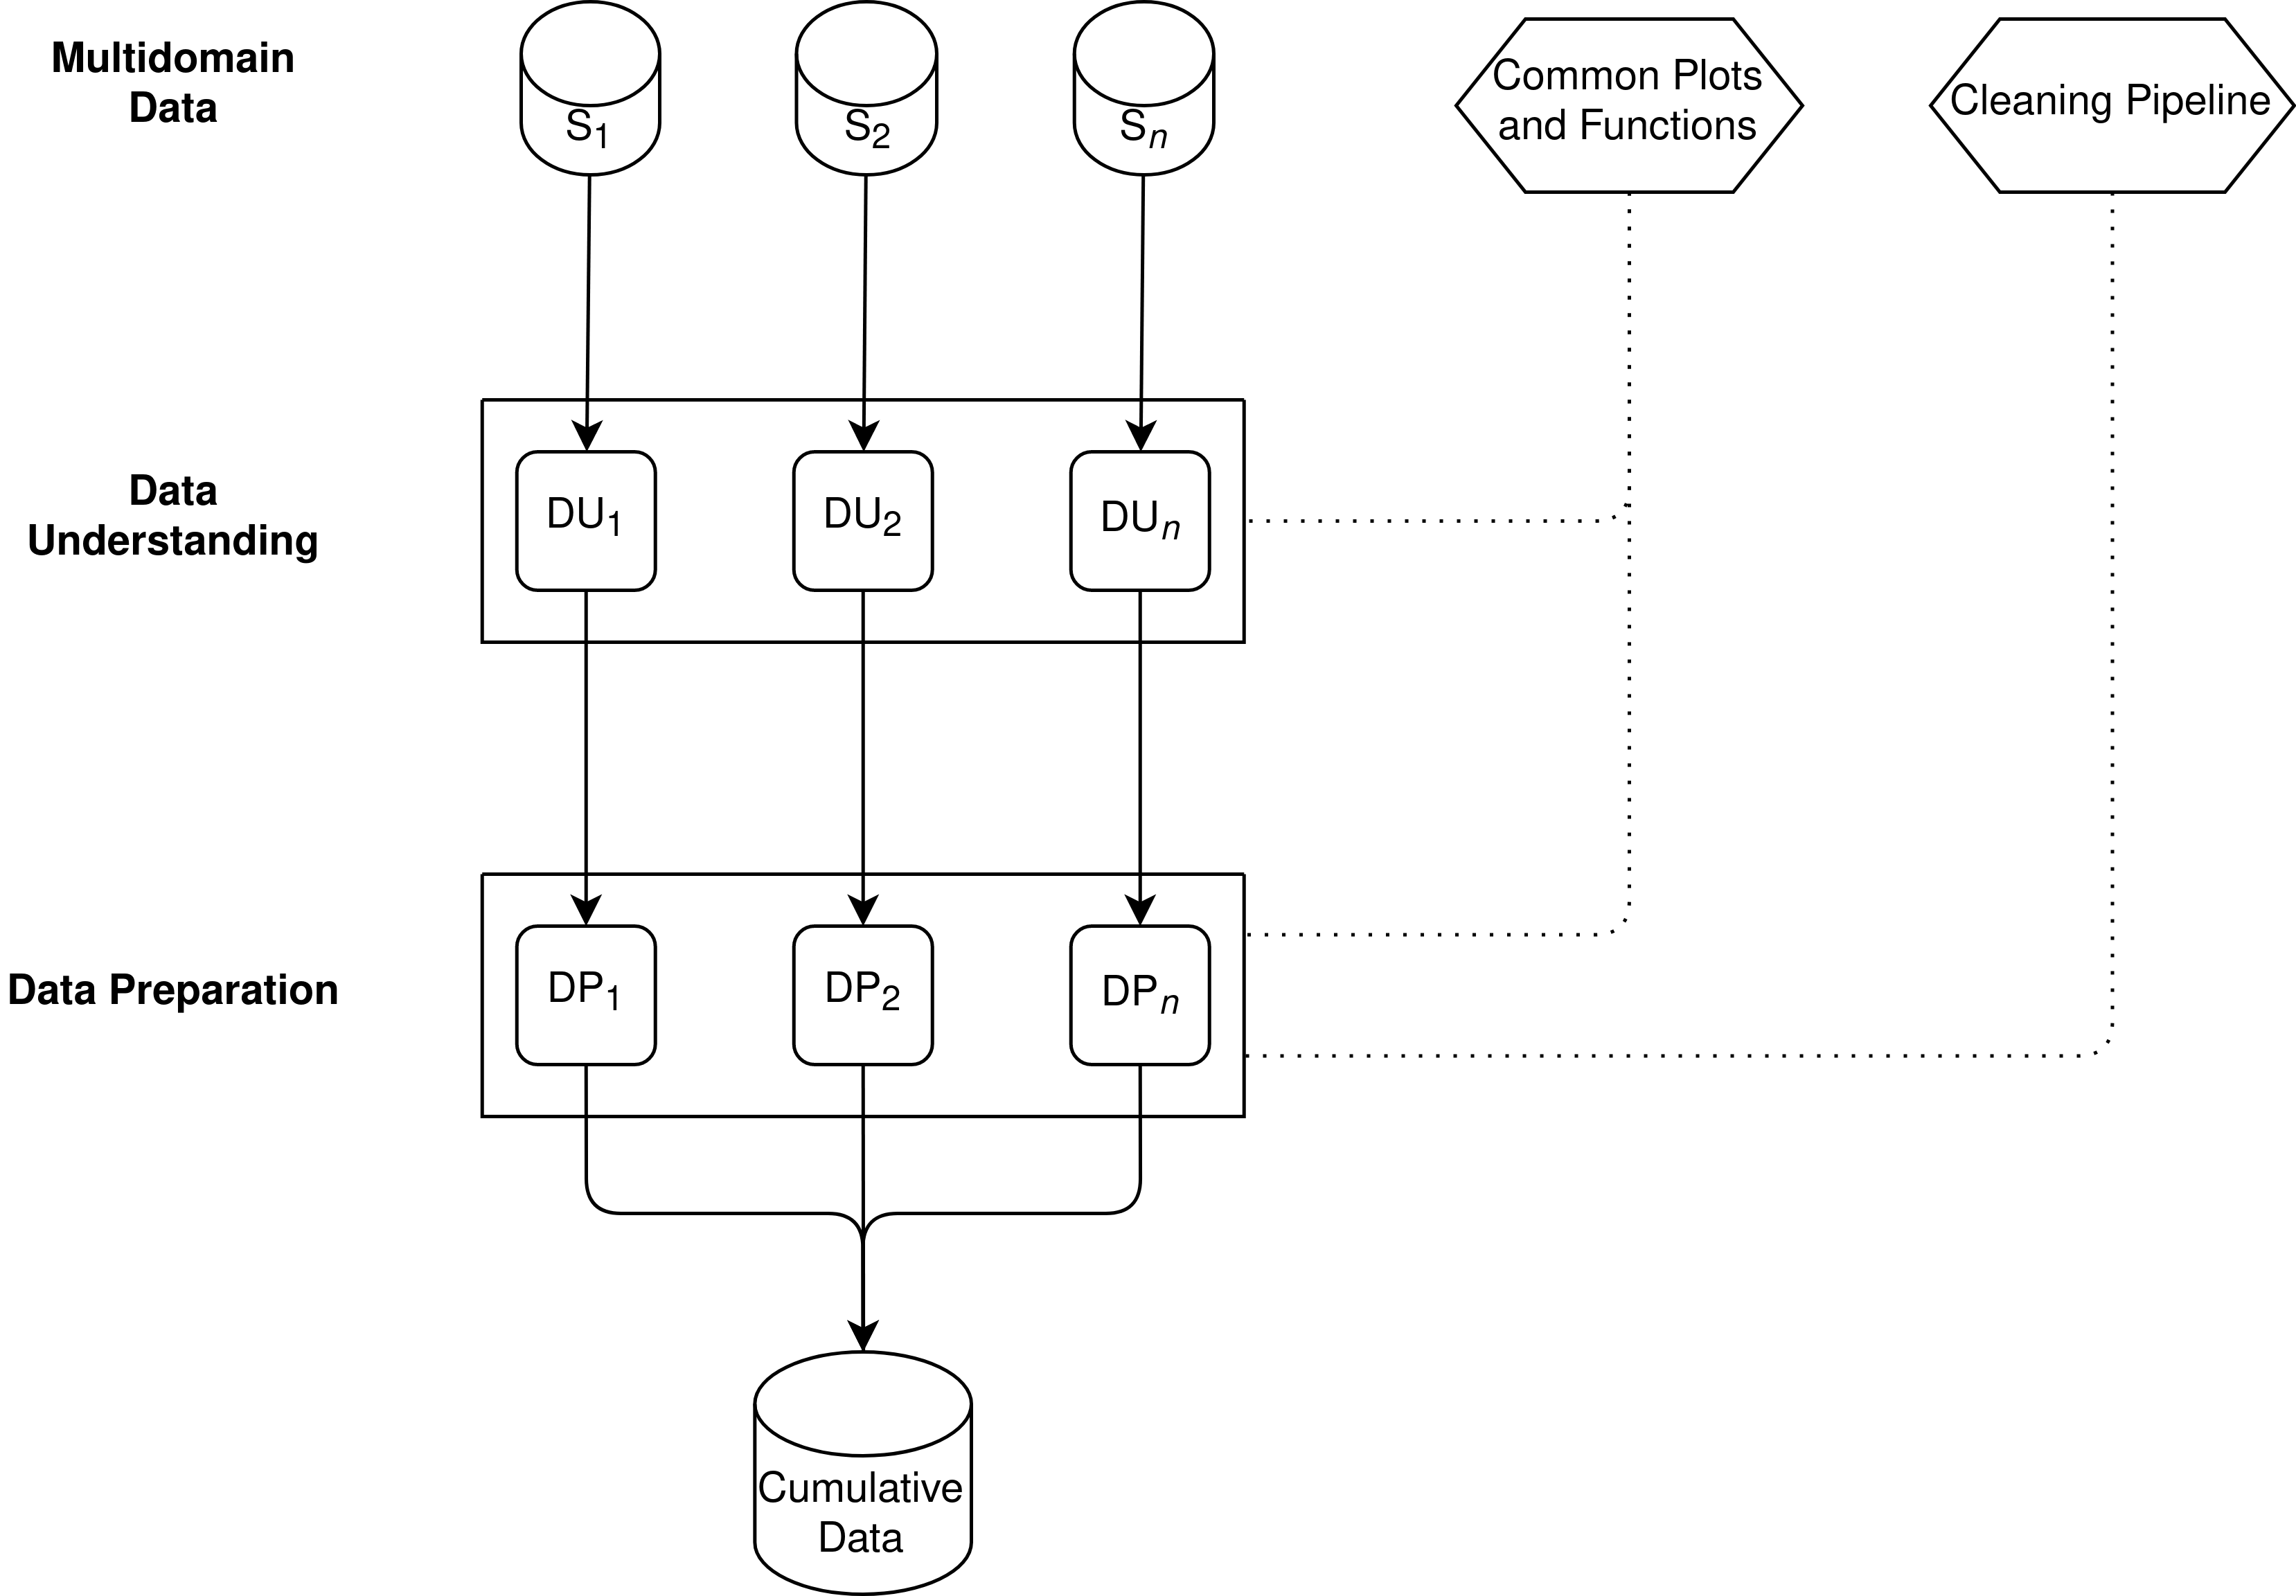
\includegraphics[width=0.7\textwidth]{data/images/data_flow_v2_1.png}
    \caption[Datenverarbeitungs-Pipeline]{Datenverarbeitungs-Pipeline} \label{fig:dataFlow_1}
\end{figure}

Mittels \autoref{fig:dataFlow_1} wird illustriert, dass die Datensätze in diesem Kapitel getrennt betrachtet und verarbeitet werden. Nachdem die Daten aufbereitet werden, können diese in \autoref{ch:crispDm_2} einzeln oder kombiniert verwendet werden.

\section{Auswahl und Sichtung der Datenquellen} \label{sec:dataUnderstanding}

Bevor näher auf die genutzten Datensätze eingegangen wird, wird umrissen, welche Anforderungen an die Auswahl dieser gelten. Im Rahmen dieser Arbeit werden ausschließlich Daten verwendet, die eindeutig Politikern aus einer der untersuchten Parteien zugeordnet werden können. Es werden alle Parteien, die wie in \autoref{subsec:btw17} beschrieben in der \num{19}. Wahlperiode im Bundestag vertreten waren, berücksichtigt. Dabei werden \ac{CDU} und \ac{CSU}, die auch eine gemeinsame Fraktion bilden, zusammen als Union betrachtet. Die Parteizuordnung ermöglicht das Trainieren von Modellen mittels Verfahren des überwachten Lernens (engl. Supervised Learning) in \autoref{ch:crispDm_2}. Ein weiteres Kriterium ist die Größe der Datensätze. Aus der Literaturrecherche in \autoref{sec:introductionTextanalysis} geht hervor, dass vergleichbare Arbeiten Datensätze mehreren Tausend bis Millionen Einträgen für Textklassifikation-Aufgaben verwenden. Des Weiteren ist darauf zu achten, dass sie die Datensätze aus einer vertraulichen Quelle stammen und eine gute Datenqualität aufweisen. Ferner ist es wichtig, dass die Lizenzen und Datenschutzbestimmungen die Nutzung der Datensätze im Rahmen dieser Arbeit erlauben. Auf Basis der Bedingungen werden drei Datensätze, bestehend aus unterschiedlichen Textsorten, gewählt. 

Bei den  gewählten Datensätzen handelt es sich um Tweets\footnote{Tweets werden von \textcite{saltzer_bundestagswahl_2022, saltzer_finding_2022, guhr_training_2020, wong_quantifying_2016} als Datensatz verwendet.}, Wahlprogramme\footnote{Wahlprogramme werden ebenfalls von \textcite{biessmann_predicting_2016} verwendet.} (Landtags-, Europa- und Bundestagswahlen) und Reden\footnote{\textcite{doan_using_2022, biessmann_predicting_2016, simoes_fine-tuned_2020} nutzen politische Reden als Datenquelle.} aus dem Deutschen Bundestag.

Die Datensätze entstammen der 19. Legislaturperiode des Deutschen Bundestages oder werden auf diese beschränkt. Das hat den Hintergrund, dass die vorkommenden Themen und Debatten in allen Datensätzen übereinstimmen sollen, damit es zu keinen Störfaktoren beim Trainieren von Klassifikatoren auf dem zusammengefügten Datensatz kommt. Die Arbeit von \textcite{richter_open_2021} legt nahe, dass Parteien über einen längeren Zeitraum ihren politischen Schwerpunkt ändern. Das führt dazu, dass die Erkennung von Strukturen in Texten erschwert wird. Diese These soll in \autoref{subsec:furtherExperiments} überprüft werden.

{\footnotesize
\begin{longtblr}[caption={Anzahl an Einträgen pro Datensatz und pro Partei vor Bereinigen und Filtern}, label={tab:countPerDataset}, note{1} = {Tweets von den aufgeführten Parteien, exklusive parteilose Politiker}, note{2} = {Reden von den aufgeführten Parteien in dem Zeitraum der 19. Legislaturperiode.},]{rowhead=1, rowfoot=1, hline{1-2, Y-Z} = {0.75pt}, colspec={l*{7}{Q[si={table-format=6},c]}}, row{1}={guard,font=\bfseries}, row{5}={font=\bfseries}}
    Datensatz & AfD & Grüne & SPD & Union & Linke & FDP & Gesamt\-anzahl \\ 

    Tweets\TblrNote{1} & 126132 & 167060 & 167647 & 157035 & 141738 & 112067 & 871679 \\
    Reden\TblrNote{2} & 4437 & 3857 & 5249 & 8007 & 3403 & 3888 & 28841 \\
    Wahlpro\-gramme & 2619 & 6399 & 4552 & 4564 & 5204 & 4376 & 27714 \\

    Summe & 133188 & 176861 & 177448 & 170246 & 150345 & 120331 & 928234 \\
\end{longtblr}
}

Die vorliegende \autoref{tab:countPerDataset} enthält statistische Informationen zu den verschiedenen Datensätzen. Insgesamt werden \num{928234} Einträge erfasst, wobei die \ac{AfD} \num{133188} Einträge, die Grünen \num{176861} Einträge, die \ac{SPD} \num{177448} Einträge, die Union \num{170246} Einträge, die Linke \num{150345} Einträge und die \ac{FDP} \num{120331} Einträge aufweisen. Der Tweet-Datensatz ist mit parteiübergreifend \num{871679} Datenpunkten mit Abstand der größte Datensatz. Der Datensatz zu den Reden enthält \num{28841} und der zu den Wahlprogrammen \num{27714} Einträge.

\subsection*{Tweets}

Twitter ist eine amerikanische Kurznachrichten-Plattform, die den Nutzern ermöglicht, Tweets von einer Länge von bis zu 280 Zeichen zu veröffentlichen. Zusätzlich zum Veröffentlichen von eigenen Tweets, besitzen Nutzer die Möglichkeit Tweets von anderen zu kommentieren, oder zu retweeten\footnote{Einen Tweet eines anderen Nutzers auf seinem eigenen Profil erneut veröffentlichen}.

Der Tweet-Datensatz von \textcite{saltzer_finding_2022} umfasst \num{876118} Tweets von \num{511} Politikern des Deutschen Bundestages zwischen Januar \num{2017} bis Dezember \num{2019}. Aufgrund der Entwicklerrichtlinien von Twitter\footnote{\href{https://developer.twitter.com/en/developer-terms/agreement}{https://developer.twitter.com/en/developer-terms/agreement}} ist der Datensatz nicht öffentlich zugänglich. \textcite{saltzer_finding_2022} hat auf Anfrage den Datensatz für diese Arbeit zur Verfügung gestellt. Dennoch erlaubt die Richtlinie die Verwendung der Daten für wissenschaftliche Analysen.

Der Datensatz beinhaltet neben den Tweet-Texten (\texttt{text}) auch noch den Twitternamen (\texttt{screen\_name}), das Erstellungsdatum (\texttt{created\_at}), ob es sich um einen Retweet handelt (\texttt{is\_retweet}), welcher Partei der Politiker angehört (\texttt{party}), das Geburtsdatum (\texttt{birthyear}) und das Geschlecht des Politikers (\texttt{gender}). Initial beinhaltet der Datensatz außerdem noch, ob der Politiker einer Untergruppierung einer Partei angehört und wie dieser bei Abstimmungen im Deutschen Bundestag abgestimmt hat. Diese letzten beiden Informationen werden jedoch im folgenden nicht weiter berücksichtigt.

Die Tweets der Parlamentarier lassen sich folgenden sechs Parteien\footnote{Initial beinhaltet der Datensatz zusätzlich Parteilose, die jedoch direkt gefiltert werden.} zuordnen: Die Grünen, \ac{SPD}, Die Linke, \ac{AfD}, \ac{FDP} und Union. Unter den \ac{MdB} befinden sich \num{161} Frauen und \num{350} Männer.

\begin{figure}[H]
    \centering
    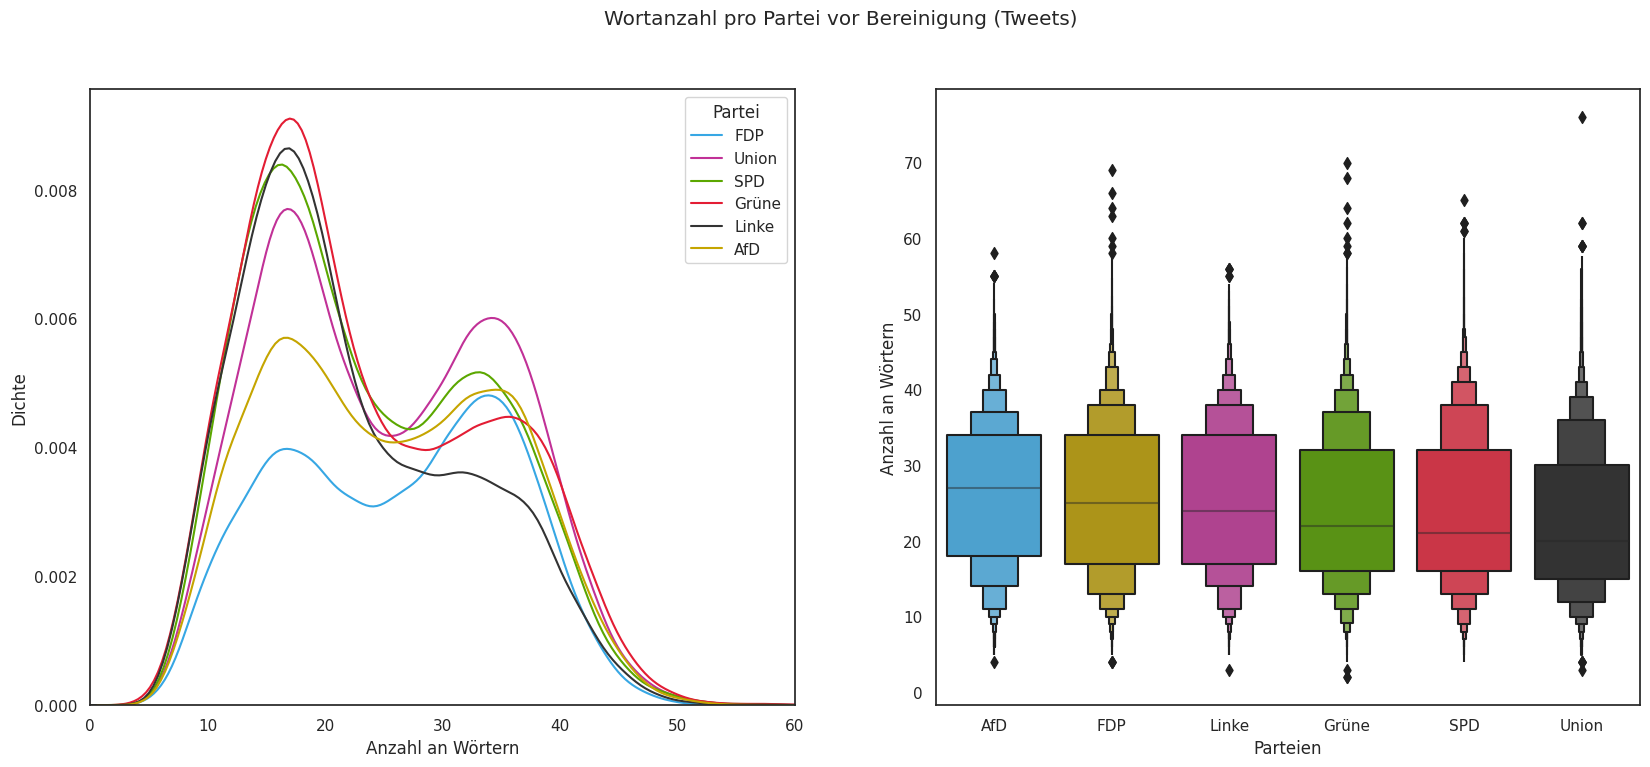
\includegraphics[width=0.9\textwidth]{data/images/tweets/wortanzahl_pro_partei_vor_bereinigung.png}
    \caption{Anzahl an Wörtern für Tweets vor Bereinigung} \label{fig:wordCountTweets}
\end{figure}

\autoref{fig:wordCountTweets} zeigt eine Dichtefunktion der Wortanzahl der Tweets gruppiert nach den einzelnen Parteien. Diese weisen jeweils zwei Extrema auf. Das Erste befindet sich im Bereich zwischen \num{15} bis \num{25} Wörtern und das Zweite im Bereich zwischen \num{30} bis \num{40} Wörtern. Im Durchschnitt veröffentlichen Politiker der Union vergleichsweise kurze Nachrichten, wohingegen die der \ac{AfD}, der \ac{FDP} und die der Linken vermehrt längere Nachrichten veröffentlichen.

\subsection*{Reden} \label{subsec:dataUnderstandingReden}

Als weitere Datenquelle sollen politische Reden, die von den Abgeordneten der verschiedenen Fraktionen im Bundestags gehalten worden sind, genutzt werden. Dabei kann auf den \enquote{Open Discourse} Datensatz von \textcite{richter_open_2021} zurückgegriffen werden, der alle Plenarprotokolle des Deutschen Bundestages von \num{1949} bis \num{2020} in Textform zur Verfügung stellt. Für den Datensatz ist die \textit{CC0 1.0} Lizenz ausgewiesen, die eine uneingeschränkte Nutzung der Daten ohne explizite Erlaubnis bietet.

Neben den Reden, die im Folgenden als Trainingsdaten genutzt werden sollen, enthält der Datensatz auch alle Zwischenrufe und -fragen, die von Parlamentariern während der Debatten geäußert wurden. Aufgrund von mangelnder Qualität und Länge dieser werden sie für den weiteren Verlauf der Arbeit als Datenquelle verworfen.

Zusätzlich zum Text (\texttt{speechContent}) liegen für jede Rede unter anderem zusätzlich die Nummer der Sitzung des Bundestages (\texttt{session}), das Datum (\texttt{date}), Vor- und Nachname (\texttt{firstName} bzw. \texttt{lastName}), die Fraktion (\texttt{factionId}) sowie die Position des Redners (\texttt{positionLong}) vor.

Über alle Wahlperioden hinweg enthält der Datensatz insgesamt \num{907644} Reden von \num{4105} Politikern. Im Rahmen dieser Arbeit werden nur Reden aus der 19. Wahlperiode berücksichtigt. Es bleiben dabei noch \num{60958} Reden in der genannten Wahlperiode übrig. Die übrigen Reden umfassen jedoch auch Beiträge des Präsidiums des Deutschen Bundestages sowie fraktionsloser Abgeordneter, die beide nicht betrachtet werden können, da sie keiner der definierten Parteien zuzuordnen sind. Somit reduziert sich die Zahl an Reden schlussendlich auf \num{28841}.

\begin{figure}[H]
    \centering
    \includegraphics[width=0.9\textwidth]{data/images/speeches/speeches_word_count.png}
    \caption{Anzahl an Wörtern für Reden vor Bereinigung} \label{fig:wordCoundSpeeches}
\end{figure}

\autoref{fig:wordCoundSpeeches} zeigt die Verteilung der Anzahl an Wörtern, die die Reden im Datensatz umfassen, aufgeschlüsselt nach Partei. Es ergibt sich dabei ein Hochpunkt in der Dichtefunktion bei knapp unter 100 Wörtern, gefolgt von einem Tiefpunkt zwischen \num{200} und \num{300} Wörtern und schließlich einem weiteren Hochpunkt, je nach Partei zwischen 400 und 700 Wörtern.

Das zeigt, dass die Reden im Durchschnitt etwa um den Faktor zehn länger sind als Tweets. Reden im Bundestag dauern oft mehrere Minuten an und können so einen ausführlichen Beitrag zu einer Debatte bringen. Bei Tweets hingegen handelt es sich um Kurznachrichten mit Zeichenlimit, die nur dazu geeignet sind, pointierte Aussagen an die Allgemeinheit zu richten.

Bei genauerer Betrachtung der Häufung von kurzen Reden rund um das erste Maximum fällt auf, dass dort viele Redebeiträge enthalten sind, die nur beispielsweise Zwischenfragen darstellen und keine vollständigen, inhaltlich relevanten Reden sind.

\subsection*{Wahlprogramme}

Zuletzt sollen auch Texte aus Wahlprogrammen der zu untersuchenden Parteien herangezogen werden. Dabei stehen im Untersuchungszeitraum die Bundestagswahlen \num{2017} und \num{2021}, die Europawahl 2019 sowie zahlreiche Landtagswahlen mit den entsprechend veröffentlichten Wahlprogrammen der Parteien zur Verfügung. Eine genaue Auflistung der verwendeten Wahlen inklusive Anmerkungen zu Wahlprogrammen, die nicht verarbeitet werden konnten, kann der \autoref{tab:overviewElectionsPartyPrograms} im Anhang entnommen werden.

Die Wahlprogramme werden von den jeweiligen Parteien explizit der Bevölkerung zur Verfügung gestellt. Zudem sind sie von öffentlichem Interesse und beinhalten keine sensiblen oder personenbezogen Informationen.

So ergibt sich eine Anzahl von insgesamt \num{83} Wahlprogrammen unterschiedlicher Parteien. Die Wahlprogramme können auf der Website der jeweiligen Partei bzw. des Landesverbandes im Fall einer Landtagswahl im \ac{PDF}-Format heruntergeladen werden. Anschließend wird der Text mittels der Python-Bibliothek \texttt{pdfminer}\footnote{\href{https://github.com/pdfminer/pdfminer.six}{https://github.com/pdfminer/pdfminer.six}} ausgelesen und verarbeitet.

Damit aus den Wahlprogrammen kohärente, kürzere Texte extrahiert werden können, wird jedes Wahlprogramm nach Absätzen unterteilt, sodass sich eine Gesamtanzahl von \num{28783} Paragraphen als Trainingsdaten vor der Bereinigung ergibt.

Neben dem Text des jeweiligen Paragraphen liegen als weitere Informationen, die während des Auslesens der Wahlprogramme gesammelt werden, die Partei, aus deren Wahlprogramm der Text entnommen wurde (\texttt{party}), die Art der Wahl (\texttt{election\_type})\footnote{Bundestags-, Europa- oder Landtagswahl} und ein Kürzel für die Wahl (\texttt{election})\footnote{Bestehend aus Art der Wahl, gegebenenfalls Bundesland und Jahr} vor.

\begin{figure}[H]
    \centering
    \includegraphics[width=0.9\textwidth]{data/images/party_programs/party_programs_word_count.png}
    \caption{Anzahl an Wörtern für Wahlprogramm-Paragraphen vor Bereinigung} \label{fig:wordCoundPartyPrograms}
\end{figure}

\autoref{fig:wordCoundPartyPrograms} zeigt die Verteilung der Anzahl an Wörtern der gewonnenen Wahlprogramm-Paragraphen pro Partei. Anders als bei den Reden zeigt sich hier eine rechtsschiefe Dichtefunktion mit nur einem Maximum bei -- je nach Partei -- etwa \num{30} bis \num{70} Wörtern pro Paragraph. Die Absätze aus Wahlprogrammen sind durchschnittlich länger als die Tweets, jedoch deutlich kürzer als die Transkripte der Bundestagsreden. 

\section{Datenaufbereitung} \label{sec:dataPreparation}

Im nächsten Schritt nach \ac{CRISP-DM} werden die Datensätze aufbereitet. Im Folgenden werden zwei Methoden verwendet, um das zu erreichen. Zum Ersten, Techniken, die die Integrität der Texte verändern. Das umfasst regelbasierte Verfahren, die Bildung von Wortstämmen und das Entfernen von Stopwörtern. Anschließend werden Eigenschaften definiert, nach welchen die Texte gefiltert werden. Hierbei wird die Integrität der Text nicht weiter beeinflusst.

\subsection{Datenbereinigungs-Pipeline} \label{subsec:cleaningPipeline}

Stopwörter, Links, Symbole und weitere Unregelmäßigkeiten (Rauschen, zu Englisch \textit{Noise}) beeinflussen die Performance von \ac{ML}-Modellen stark \autocite[4]{kowsari_text_2019}. Daher ist es notwendig Texte mittels regelbasierten Verfahren, als auch mit \ac{ML}-Verfahren zu bereinigen. 

\begin{figure}[H]
    \centering
    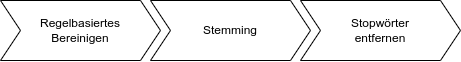
\includegraphics[width=0.7\linewidth]{data/images/cleaning_pipeline_v1.png}
    \caption{Datenbereinigungsprozess} \label{fig:cleaningPipeline}
\end{figure}

Wie \autoref{fig:cleaningPipeline} zeigt, besteht der Prozess zur Datenbereinigung aus drei Abschnitten. Zuerst die regelbasierte Bereinigung, die mittels regulären Ausdrücken und Patterns eine erste Umformung vornimmt. Im nächsten Schritt werden die Wörter auf ihren Wortstamm zurückgeführt. Im letzten Schritt werden Stopwörter entfernt. All diese Schritte verfolgen das Ziel, die Menge an Rauschen zu verringern. 

\subsubsection{Regelbasierte Verfahren}

Unterschiedliche Schreibweisen, Symbole und Emojis, \acp{URL}, und Gendern stellen ein elementares Problem für herkömmliche \ac{NLP} Methoden und Modelle dar \autocite[4\psq]{kowsari_text_2019}. Im ersten Schritt werden daher regelbasierte Verfahren genutzt, um häufig auftretende Zeichen, Symbole/Emojis, aber auch andere Unregelmäßigkeiten ersetzt oder entfernt.

Besonders bei Tweets werden häufig Symbole wie \euro~und \& als Kurzform verwendet. Die Symbole als auch die Zahlen werden mit ihrem ausgeschriebenen Klartext ersetzt, da sie nicht in dieser Form interpretiert werden können. So wird aus \euro~\(\rightarrow\) \textit{euro}, oder aus \(\num{2000} \rightarrow\) \textit{zweitausend}.

In den Texten treten vermehrt Unicode, Emojis, als auch weitere Symbole auf. In Tweets als auch in Wahlprogrammen werden ebenfalls \acp{URL} verwendet. Tweets nutzen außerdem Referenzen zu Twitternutzern (Erwähnungen wie \textit{@MaxMustermann}). Diese müssen entfernt werden, da sie nicht in dieser Form interpretiert werden können.

Bei allen Textformen verwenden Politiker und Parteien unterschiedliche Arten von inklusiver Sprache als Alternative zum generischen Maskulinum. Beispiele hierfür sind \textit{Politiker*innen} oder auch \textit{Politiker:innen}. Es  werden alle herkömmlichen Endungen für gendergerechte Sprache entfernt, da die Textrepräsentationsformen und Sprachmodelle das nur rudimentär oder gar nicht abbilden können. Folglich können alle Wörter im Text auf den korrekten Wortstamm reduziert werden.

Nach der groben Bereinigung der Texte werden letztlich noch Satzzeichen, Sonderzeichen und einzelne Buchstaben entfernt. Abschließend werden doppelte Leerzeichen entfernt und alle Buchstaben zu Kleinbuchstaben umgewandelt.

\begin{example}[H]
    {\footnotesize
    \begin{subexample}{0.45\textwidth}
        \textcolor{orange}{Ehemalige} \textcolor{red}{@AfD-Vorsitzende} \textcolor{orange}{\#Petry} muss wegen \textcolor{orange}{Meineid} vor \textcolor{orange}{Gericht}\textcolor{red}{.} \textcolor{orange}{Kein Einzelfall}\textcolor{red}{:} gegen circa \textcolor{orange}{\SI{10}{\percent}} aller \textcolor{orange}{AfD-Abgeordneten} bundesweit laufen oder liefen \textcolor{orange}{Strafverfahren}\textcolor{red}{.} \textcolor{orange}{Kriminelle Asylbewerber}\textcolor{red}{?} \textcolor{orange}{Fehlanzeige}\textcolor{red}{.} \textcolor{orange}{Kriminelle AfD-Hetzer} trifft den \textcolor{orange}{Nagel} eher auf den \textcolor{orange}{Kopf} \textcolor{red}{<U+0001F602>} \textcolor{orange}{\#AfD}
        \caption{Tweet vor jeglicher Bereinigung \parencite{saltzer_finding_2022}}
    \end{subexample}\hfill
    \begin{subexample}{0.45\textwidth}
        ehemalige petry muss wegen meineid vor gericht kein einzelfall gegen circa zehn prozent aller afd abgeordneten bundesweit laufen oder liefen strafverfahren kriminelle asylbewerber fehlanzeige kriminelle afd hetzer trifft den nagel eher auf den kopf afd
        \caption{Tweet nach regelbasierter Bereinigung}
    \end{subexample}\hfill
    }
    \caption[Beispiel -- Regelbasierte Bereinigung]{Beispiel für regelbasierte Bereinigung eines Tweets von \textit{victorperli} \autocite{saltzer_finding_2022}} \label{list:rulebasedCleaning}
\end{example}

\autoref{list:rulebasedCleaning} zeigt die Anwendung der regelbasierten Bereinigung auf einen Beispiel-Tweet. Es kann erkannt werden, dass die Referenz \textit{@AfD-Vorsitzende} im bereinigten Text nicht mehr vorkommt. Zudem wird das Hashtag-Symbol vor \textit{Petry} und \textit{AfD} entfernt. Auch die Angabe \textit{10\%} wird durch die Bereinigung ausgeschrieben zu \textit{zehn prozent}. Schließlich enthält der bereinigte Text auf der rechten Seite keine Satzzeichen mehr, das Emoji am Ende fehlt und alle Wörter sind kleingeschrieben, sodass nur noch korrekte Wörter vorkommen.

Bei den Redetexten ist zusätzlich zu beachten, dass im Datensatz Zwischenrufe von anderen Politikern im Redetext durch Referenzen -- gekennzeichnet durch eine Zahl innerhalb geschweifter und normaler Klammern -- vorkommen. Referenzen zu den Zwischenrufen werden mithilfe eines regulären Ausdrucks entfernt, da der Text nur den Inhalt der Rede selbst beinhalten soll.

Bei dem Auslesen der Wahlprogramme werden die Paragraphen nach Leerzeilen getrennt, wobei manche Absätze allerdings über das Seitenende hinaus weitergehen. Daher werden Paragraphen, die nicht mit einem Satzzeichen enden, mit darauffolgenden Paragraphen zusammengefügt. Zudem kommt es bei einigen Dokumenten dazu, dass Text aus der Kopf- und Fußzeile sowie von Anmerkungen an der Seite des regulären Textes mit ausgelesen wird. Dieser ist ungewollt in den übrigen Abschnitten enthalten und muss folglich im Rahmen der regelbasierten Bereinigung entfernt werden.

\subsubsection{Wortstamm}

Der nächste Schritt dient dazu, die Wörter zu vereinheitlichen. Hierfür werden Wörter mit dem dazugehörigen Wortstamm ersetzt (\textit{eng. Lemmatizing}). Für die Umwandelung wird \texttt{spacy}\footnote{\href{https://spacy.io/}{https://spacy.io/}} verwendet.

\begin{example}[H]
    {\footnotesize
    \begin{subexample}{0.45\textwidth}
        \textcolor{orange}{ehemalige} petry muss wegen meineid vor gericht kein einzelfall gegen circa zehn prozent aller afd \textcolor{orange}{abgeordneten} bundesweit laufen oder liefen \textcolor{orange}{strafverfahren} \textcolor{orange}{kriminelle} asylbewerber \textcolor{orange}{fehlanzeige} \textcolor{orange}{kriminelle} afd hetzer \textcolor{orange}{trifft} \textcolor{orange}{den} nagel eher auf den kopf afd
        \caption{Tweet nach regelbasierter Bereinigung}
    \end{subexample}\hfill
    \begin{subexample}{0.45\textwidth}
        ehemalig petry muss wegen meineid vor gericht kein einzelfall gegen circa zehn prozent aller afd abgeordneter bundesweit laufen oder laufen strafverfahr kriminell asylbewerber fehlanzeig kriminell afd hetzer treffen der nagel eher auf der kopf afd
        \caption{Tweet nach dem Bilden der Wortstämme}
    \end{subexample}\hfill
    }
    \caption[Bildung von Wortstämmen]{Beispiel für die Bildung von Wortstämmen eines Tweets von \textit{victorperli} \autocite{saltzer_finding_2022}} \label{list:lemma}
\end{example}

\autoref{list:lemma} veranschaulicht, dass unter anderem Endungen wie \textit{e} und \textit{en} mit dem jeweiligen Stamm ersetzt werden. Wenn Wörter nicht in dem Wörterbuch enthalten sind, werden diese exkludiert.

\subsubsection{Stopwörter}

Stopwörter sind Füllwörter, die keine starke Relevanz für die Bedeutung eines Satzes haben \autocite[4]{kowsari_text_2019}. Das dadurch entstehende Rauschen kann unterdrückt werden, indem die Stopwörter gefiltert werden.

\begin{example}[H]
    {\footnotesize
    \begin{subexample}{0.45\textwidth}
        ehemalig petry \textcolor{red}{muss wegen} meineid \textcolor{red}{vor} gericht \textcolor{red}{kein} einzelfall \textcolor{red}{gegen} circa zehn prozent \textcolor{red}{aller} afd abgeordneter bundesweit laufen \textcolor{red}{oder} laufen strafverfahr kriminell asylbewerber fehlanzeig kriminell afd hetzer treffen \textcolor{red}{der} nagel eher \textcolor{red}{auf der} kopf afd
        \caption{Tweet nach dem Bilden der Wortstämme}
    \end{subexample}\hfill
    \begin{subexample}{0.45\textwidth}
        ehemalig petry wegen meineid gericht einzelfall circa zehn prozent afd abgeordneter bundesweit laufen laufen strafverfahr kriminell asylbewerber fehlanzeig kriminell afd hetzer treffen nagel eher kopf afd
        \caption{Tweet nach dem Entfernen von Stopwörtern}
    \end{subexample}\hfill
    }
    \caption[Beispiel -- Entfernen von Stopwörtern]{Beispiel für das Entfernen von Stopwörtern eines Tweets von \textit{victorperli} \autocite{saltzer_finding_2022}} \label{list:stopwords}
\end{example}

Für das Filtern, wie in \autoref{list:stopwords} gezeigt, wird das Stoppwort-Lexikon von \texttt{nltk}\footnote{\href{https://www.nltk.org/}{https://www.nltk.org/}} für die deutsche Sprache verwendet. Wie aus dem Beispiel hervorgeht, werden häufig auftretende Wörter ohne stärkeren Kontext und ohne Bedeutung für den zentralen Sinn des Textes entfernt.

\subsection{Filtering} \label{subsec:filtering}

Auf Basis der Erkenntnisse aus \nameref{sec:dataUnderstanding} werden im Folgenden die Datensätze gefiltert. Das ist wichtig, um die Datenqualität zu erhöhen und etwaige Bias zu vermeiden.

\subsubsection*{Tweets} \label{subsubsec:filteringTweets}

Der Tweet-Datensatz \textcite{saltzer_finding_2022} weist Tweet-Duplikate auf. Diese sind jeweils von dem gleichen Politiker verfasst und weisen den gleichen Text auf. Lediglich das Erstellungsdatum (\texttt{created\_at}) des Eintrages weicht bei den Duplikaten voneinander ab. Aufgrund der Indikation eines Fehlers beim Data-Mining erfolgt die Beibehaltung lediglich der jüngsten Einträge dieser Duplikate.

Des Weiteren existieren Einträge, bei denen der Tweet-Text als auch das \texttt{is\_retweet} Label, leer ist. Diese Einträge werden ebenfalls komplett entfernt, da beide Datenpunkte benötigt werden. 

Tweets, die lediglich von Politikern erneut geteilt werden, lassen sich nicht eindeutig dem Politiker selbst und seinen Ansichten zuordnen. Es könnte also sein, dass ein Politiker einen Tweet entweder retweetet, weil er der Aussage und Meinung zustimmt, oder auch falls er komplett andere Ansichten hat und seine Reichweite nutzen möchte, um Aufmerksamkeit auf den Autor und das Thema zu lenken. Aufgrund dieser Ungewissheit werden Tweets, die als Retweet gegengezeichnet werden, entfernt.

\autoref{fig:wordCountTweets} bestätigt, dass vermehrt kurze Tweets (\numrange{15}{25}) und lange Tweets (\numrange{30}{40}) veröffentlicht werden. Bei Tweets mit weniger als \num{10} Wörtern ist es schwierig, einen tieferen Kontext festzustellen. Daher werden diese Tweets, entfernt (\texttt{stemm\_text >= 10}).

\subsubsection*{Reden}

Gemäß den Feststellungen in \autoref{subsec:dataUnderstandingReden} beinhaltet der Datensatz von \citeauthor{richter_open_2021} nicht nur Reden zur 19. Wahlperiode des Deutschen Bundestages, sondern auch ältere Reden. Daher muss der Datensatz in einem ersten Schritt auf den entsprechenden Untersuchungszeitraum begrenzt werden.

Ferner können als Trainingsdaten für das Klassifikationsmodell nur Texte verwendet werden, die einer der sechs Fraktionen im Bundestag zuzuordnen sind. Daher müssen auch Redebeiträge von fraktionslosen Abgeordneten sowie des Präsidiums ausgeschlossen werden.

Bei der Betrachtung der Anzahl an Wörtern in Reden (siehe \autoref{subsec:dataUnderstandingReden}) ist aufgefallen, dass es eine Häufung von vergleichsweise kurzen Texten mit einer Länge von unter \num{200} Wörtern gibt. Bei diesen kann nicht sichergestellt werden, dass sie ausreichend politischen Inhalt bieten, als auch der Kontext der Aussagen klar wird. Deshalb werden im weiteren Verlauf nur noch Reden mit mindestens 200 Wörtern berücksichtigt (\texttt{word\_count >= 200}).

Es ist erforderlich, lange Reden in mehrere kleinere Textabschnitte aufzuteilen, damit die Texte ohne Probleme von vortrainierten Sprachmodellen als Eingabe genutzt werden können. Anderenfalls besteht die Gefahr, die maximale Anzahl an Eingabe-Tokens\footnote{Bei \ac{BERT}-basierten Modellen, die für das Modeling genutzt werden sollen, sind es maximal \num{512} Tokens.} zu überschreiten. Dabei wird darauf geachtet, dass eine Rede nur nach einem abgeschlossenen Satz aufgetrennt wird, um die Qualität der Daten nicht zu verringern.

Der Datensatz enthält außerdem drei Einträge mit dupliziertem Text, die daher ausgeschlossen werden.

\subsubsection*{Wahlprogramme}

Einträge aus einem falschen Zeitraum oder von einer nicht zu untersuchenden Partei kommen im Wahlprogramm-Datensatz nicht vor, da die Daten zu den Wahlprogrammen selbst gesammelt und verarbeitet werden.

Bereits im Zuge des Auslesens der \ac{PDF}-Dateien der Wahlprogramme werden nur Absätze mit mindestens \num{150} Zeichen weiterverarbeitet. Bei Absätzen mit weniger Zeichen handelt es sich mehrheitlich um kurze Überschriften. Die Abschnitte sind im Vergleich zu den Reden deutlich kürzer. Somit ist keine Obergrenze für die Länge nötig, um die weitere korrekte Verarbeitung zu garantieren.

Auch bei den Wahlprogramm-Texten lassen sich einige Duplikate finden, die herausgefiltert werden müssen.


\section{Aufbereitete Datensätze} \label{sec:processedDataframes}

Nach Anwendung der Datenbereinigungs-Pipeline bleiben im Gesamt-Datensatz etwa \num{395000} Einträge übrig (siehe \autoref{tab:countPerDatasetAfterCleaning}). Damit reduziert sich die Größe des Datensatzes stark, da viele ursprüngliche Tweets nicht mehr enthalten sind. \autoref{tab:countPerDatasetAfterCleaning} zeigt die Anzahl an Einträgen in den drei Datensätzen sowie pro Partei.

\begin{table}[H]
    \centering\footnotesize
    \caption{Anzahl an Einträgen pro Datensatz und pro Partei nach Bereinigen und Filtern} \label{tab:countPerDatasetAfterCleaning}
    {\footnotesize
    \begin{tblr}{width=\textwidth, hline{1-2, Y-Z} = {0.75pt}, colspec={l*{7}{Q[si={table-format=6},c]}}, row{1}={guard,font=\bfseries}, row{5}={font=\bfseries}}
        Datensatz & AfD & Grünen & SPD & Union & Linke & FDP & Gesamt\-anzahl \\ 

        Tweets & 39840 & 60390 & 62227 & 54391 & 59473 & 50304 & 326625 \\*
        Reden & 5750 & 4745 & 8015 & 12209 & 4558 & 4983 & 40260 \\*
        Wahlpro\-gramme & 2618 & 6398 & 4552 & 4560 & 5203 & 4343 & 27674 \\*

        Summe & 48208 & 71533 & 74794 & 71160 & 69234 & 59630 & 394559 \\
    \end{tblr}
    }
\end{table}

Im Folgenden werden die Texte und weitere Features der Tweets, Reden und Wahlprogramme genauer untersucht. Das umfasst unter anderem eine Analyse des Sentiments mit dem Modell von \textcite{guhr_training_2020} aus \autoref{sec:sentimentanalysis}. Im Gegensatz zum Stand vor der Bereinigung ist es an dieser Stelle möglich, die Texte ohne signifikante Beeinflussung durch nicht verarbeitbaren Zeichen oder falsche Einträge zu analysieren, um erste Erkenntnisse und Unterschiede zwischen den Parteien zu identifizieren.

\subsection*{Tweets}

Entsprechend der Erläuterungen in \autoref{subsubsec:filteringTweets} werden Duplikate, Retweets und zu kurze Tweets entfernt. Aus \autoref{tab:countPerDatasetAfterCleaning} geht hervor, dass sich die Anzahl an Tweets um \SI{62.53}{\percent} reduziert.

\begin{figure}[H]
    \centering
    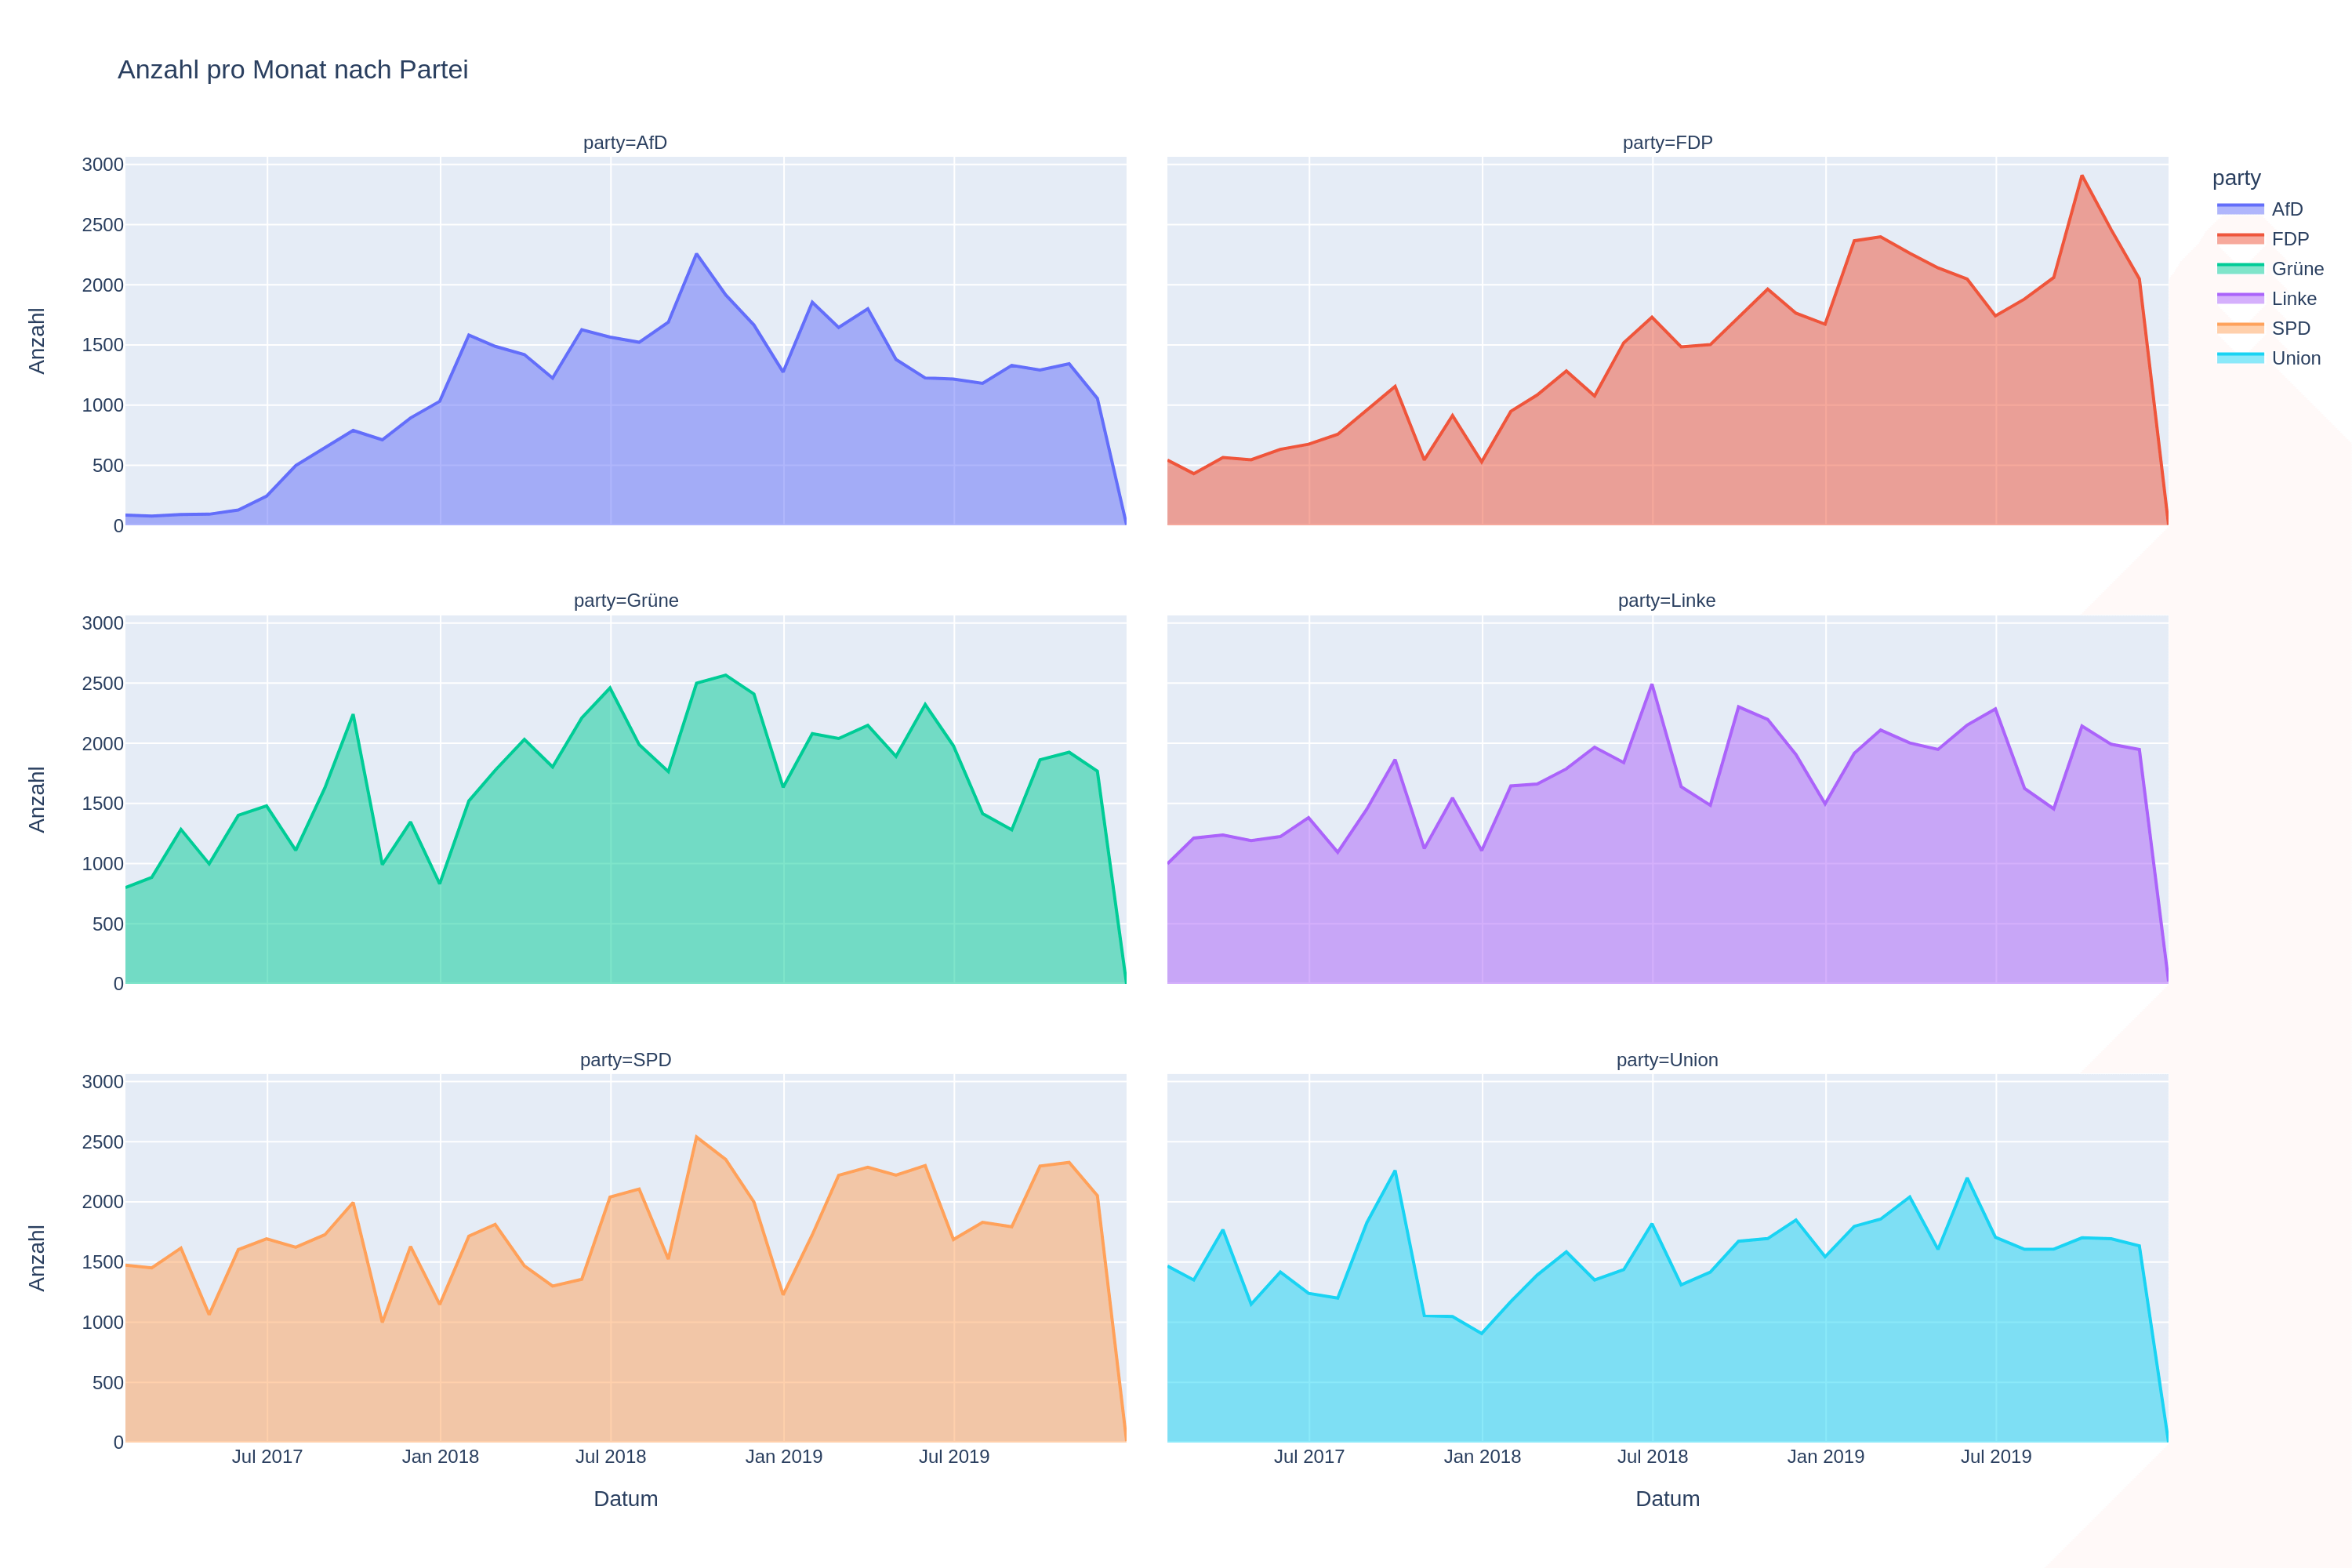
\includegraphics[width=\textwidth]{data/images/tweets/anzahl_pro_monat_nach_partei.png}
    \caption{Anzahl an Tweets pro Monat nach Partei} \label{fig:countTweetsTimeline}
\end{figure}

In der \autoref{fig:countTweetsTimeline} weisen besonders zwei Parteien, in dem Betrachtungszeitraum, einen starken Trend in der Anzahl an Tweets pro Partei ab.

Zum einen die \ac{AfD}, von der vor dem Jahr \num{2017} wenige Tweets vorhanden sind. Wie in \autoref{subsec:btw17} dargelegt, ist die \ac{AfD} erst durch die Bundestagswahl \num{2017} in den Bundestag eingezogen. Vor der Bundestagswahl \num{2017} umfasst der Datensatz von \textcite{saltzer_bundestagswahl_2022} \num{31} \ac{AfD}-Politiker, während nach der Bundestagswahl insgesamt \num{74} enthalten sind. Es ist naheliegend, dass manche Abgeordneten erst nach dem Einzug in den Bundestag angefangen haben, Twitter aktiv zu nutzen. Der starke Zuwachs der \ac{AfD} flacht ab Januar \num{2018} ab. Von da an enthält der Datensatz im Durchschnitt \num{1433} im Namen der \ac{AfD}.

Weiterhin ist ebenfalls der Verlauf der \ac{FDP} auffällig. Diese weist einen starken Zuwachs an Tweets über den gesammelten Zeitraum auf. Aus der \autoref{fig:countTweetsTimeline} geht hervor, dass zu Anfang die \ac{FDP} circa \num{500} Tweets abgesetzt hat und gegen Ende rund \numrange{2500}{3000}. Das entspricht einem monatlichen Zuwachs von \SI{4.36}{\percent}.

Bei den Grünen lässt sich eine leichte Zunahme in der Anzahl in der Mitte des Zeitraums feststellen. Über den gesamten Zeitraum werden durchschnittlich pro Monat \num{1725} Tweets abgesetzt. Die Linke, \ac{SPD} und Union sind nicht weiter auffällig, mit der Ausnahme von einzelnen lokalen Extrema. Von den drei Parteien tweetet die \ac{SPD} mit \num{1728} am meisten, gefolgt von der Linken mit \num{1652} und der Union mit \num{1510} Tweets pro Monat.

\begin{table}[H]
    \centering
    \caption{Prozentuale Sentimentverteilung von Tweets pro Partei} \label{tab:sentimentDistributionTweet}
    {\footnotesize
    \begin{tblr}{width=\textwidth, hline{1-2, Z} = {0.75pt}, colspec={l*{3}{Q[si={table-format=1.2},c]}}, row{1}={guard,font=\bfseries,l}} 
        Partei & Negative & Neutral & Positive \\
        
        AfD & 0.28 & 0.68 & 0.04 \\
        Die Grüne & 0.20 & 0.74 & 0.06 \\
        Die Linke & 0.21 & 0.75 & 0.04 \\
        FDP & 0.22 & 0.73 & 0.05 \\
        \hline
        SPD & 0.18 & 0.74 & 0.09 \\
        Union & 0.16 & 0.78 & 0.07 \\
    \end{tblr}
    }
\end{table}

Auffällig bei den Tweets ist, dass besonders die Regierungsparteien -- Union und \ac{SPD} -- sich weniger negativ äußern als die Oppositionsparteien. Bei den positiven Tweets zeigt sich ein invertiertes Verhalten, wobei allgemein die Rate an positiven Tweets deutlich geringer ist.

\begin{figure}[H]
    \centering
    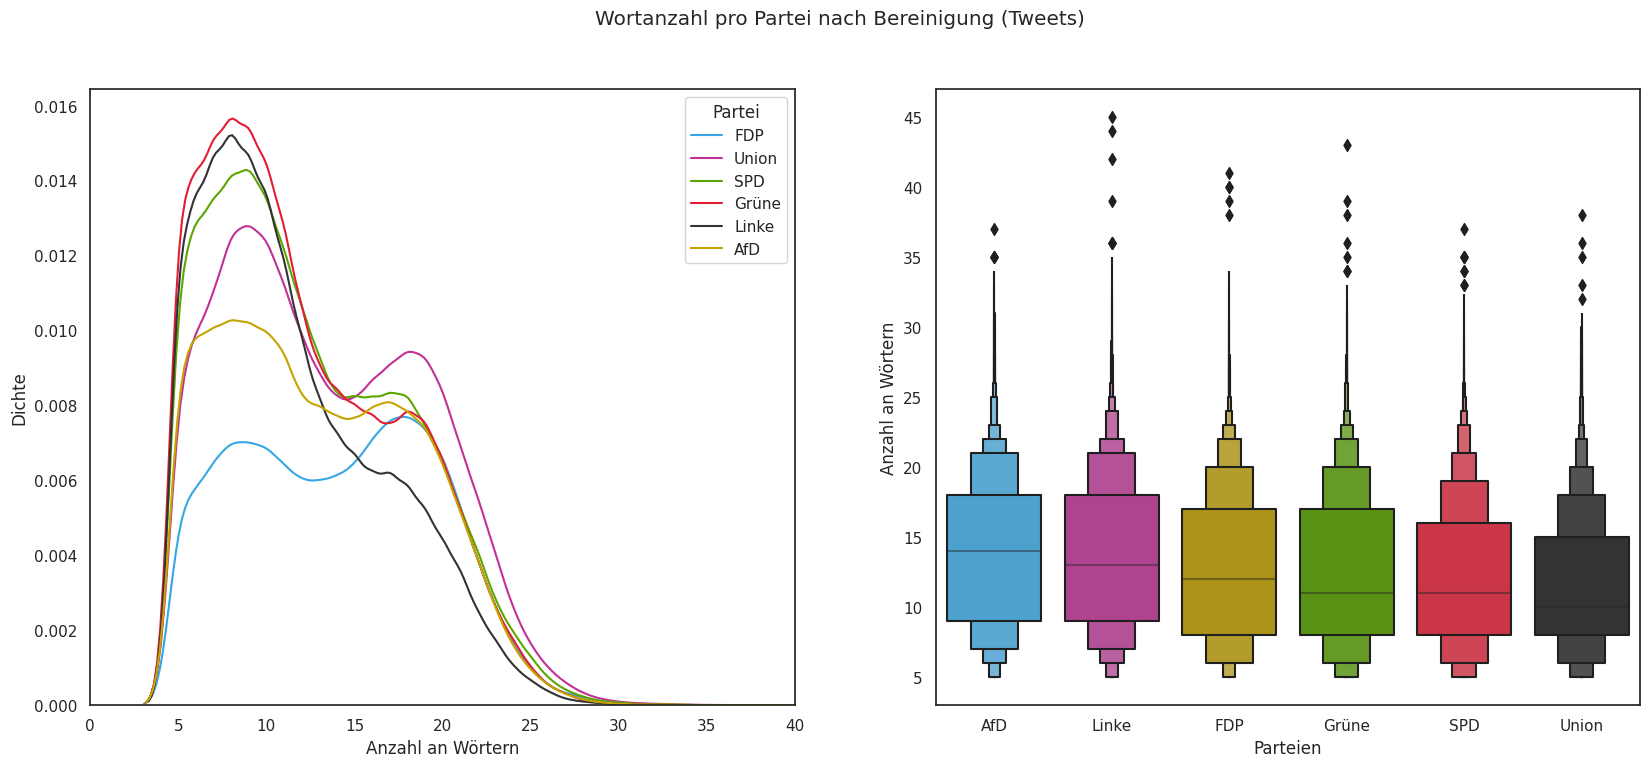
\includegraphics[width=\linewidth]{data/images/tweets/wortanzahl_pro_partei_nach_bereinigung.png}
    \caption{Wortanzahl pro Partei nach Bereinigung} \label{fig:countPartyCleaned}
\end{figure}

Eine genaue Analyse von \autoref{fig:wordCountTweets} verdeutlicht, dass die Tweets nach der Bereinigung in \autoref{fig:countPartyCleaned} zwei Maxima aufweisen. Durch das Entfernen von Wörtern und Endungen verringert sich die durchschnittliche Länge der Tweets. Die neuen Hochpunkte befinden sich bei \num{10} und \num{20} Wörtern. Auffällig ist, dass bei allen Parteien, außer der \ac{AfD}, das erste Maximum stärker ausgeprägt ist. Bei der \ac{AfD} ist somit der Anteil an Tweets mit mehr Wörtern höher.

\begin{figure}[H]
    \centering
    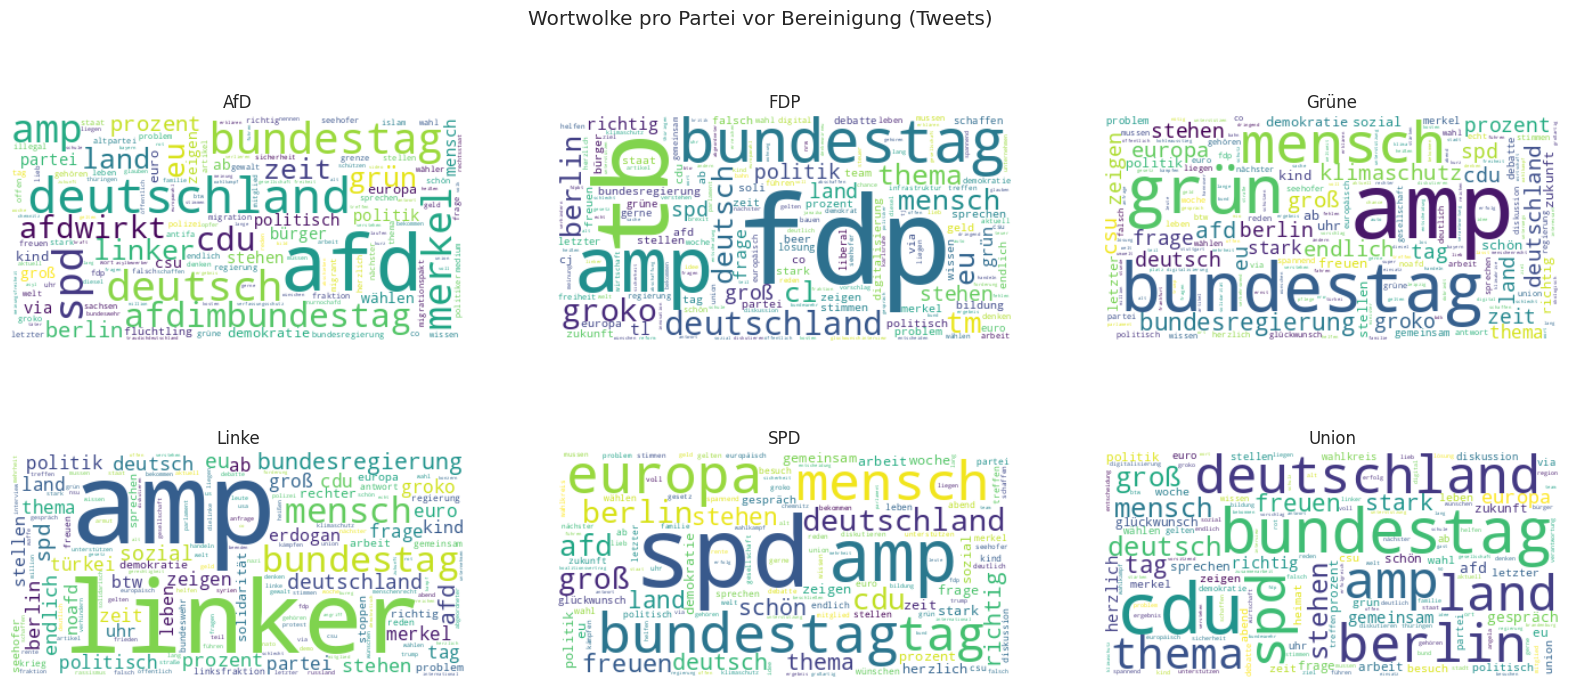
\includegraphics[width=\linewidth]{data/images/tweets/wortwolke_pro_partei_vor_bereinigung.png}
    \caption{Wortwolken mit den meistgenutzten Wörtern in Tweets pro Partei} \label{fig:tweetsWordclouds}
\end{figure}

\autoref{fig:tweetsWordclouds} visualisiert die häufigsten Wörter gruppiert nach den sechs Parteien als Wortwolken. Bei der \ac{AfD} stechen Wörter wie \textit{deutschland} und \textit{merkel} hervor. Zusätzlich werden Wörter wie \textit{islam}, \textit{antifa} und \textit{flüchtling} oft genutzt. Die \ac{FDP} verwendet häufig Wörter wie \textit{groko}, \textit{mensch}, \textit{bundestag} und \textit{cl} (Abkürzung für Christian Lindner). Darüber hinaus treten \textit{geld}, \textit{bürger} und \textit{infrastruktur} auf. Die Grünen neigen dazu, besonders stark Wörter wie \textit{grün} und \textit{mensch} zu verwenden. Außerdem tauchen ebenfalls Wörter wie \textit{klimaschutz}, \textit{zukunft}, \textit{kind} und \textit{sozial} auf. Bei den Linken dominiert \textit{linker}. Weitere Wörter sind \textit{sozial}, \textit{noafd}, \textit{türkei} und \textit{frage} auf. Die \ac{SPD} hingegen verwendet Wörter wie \textit{eurpoa}, \textit{mensch}, \textit{sozial} und \textit{schön}. Die Union fällt mit Wörtern wie \textit{stark}, \textit{groß}, \textit{arbeit} und \textit{wahlkreis} auf.

Die Texte der jeweiligen Parteien weisen am häufigsten eigene Parteinamen oder thematische Synonyme auf. Weiterhin lassen sich Zusammenhänge zu den Standpunkten der Parteien aus \autoref{subsec:heterogenitätParteien} feststellen.

\subsection*{Reden}

Auf den ersten Blick fällt auf, dass die Anzahl der Reden nach dem Bereinigungs- und Filterprozess deutlich gestiegen ist. Das lässt sich darauf zurückführen, dass viele der Reden zu lang sind und aufgeteilt werden, um die maximale Anzahl an Tokens nicht zu überschreiten. Daraus resultiert, dass es mehrere Einträge in dem Datensatz gibt, die auf die gleiche Rede zurückzuführen sind.

\begin{figure}[H]
    \centering
    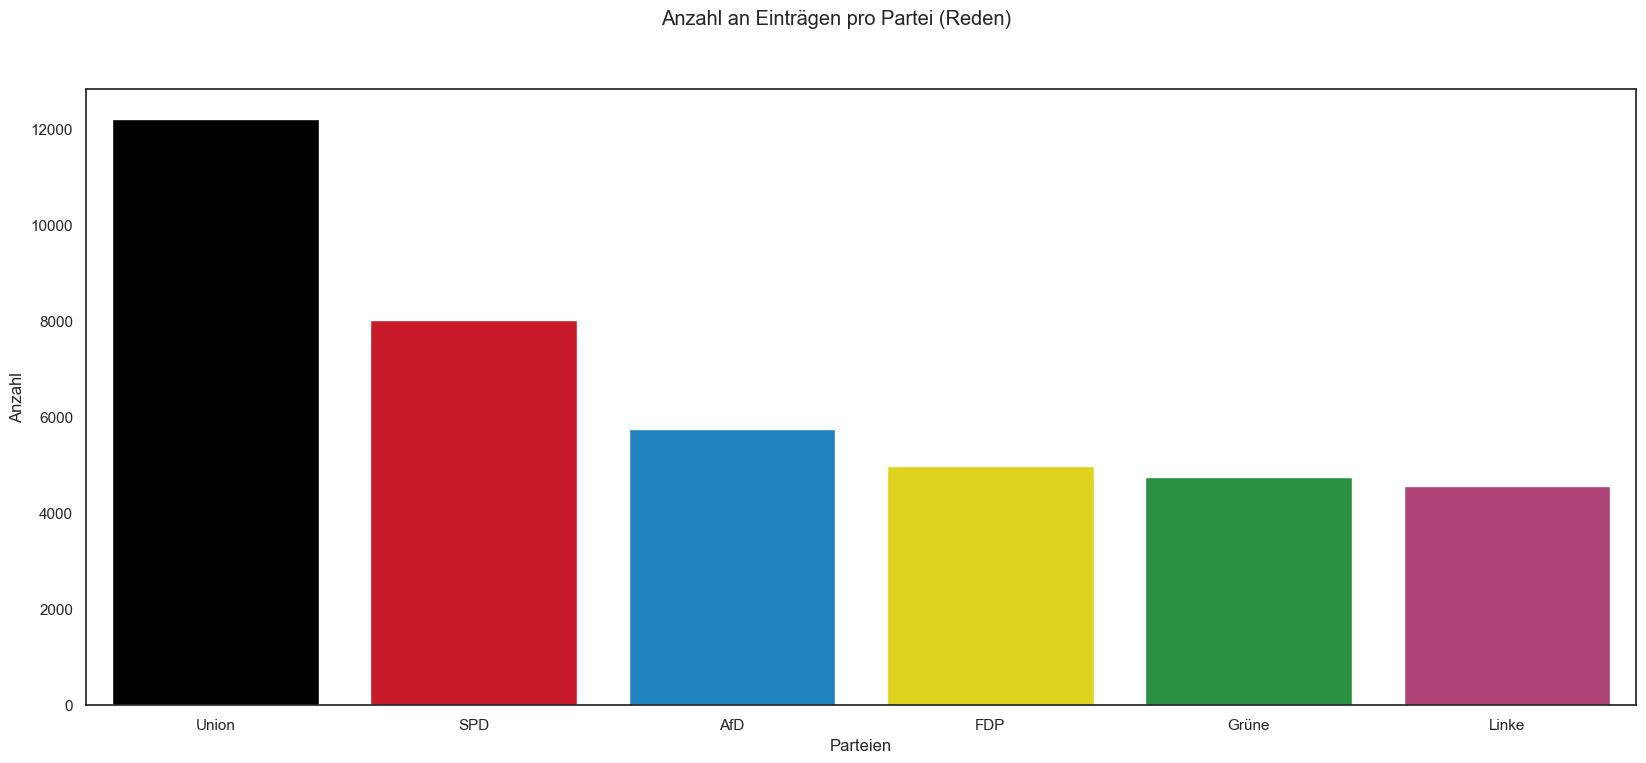
\includegraphics[width=0.9\textwidth]{data/images/speeches/speeches_num_samples_after_filter.png}
    \caption{Anzahl an Einträgen für Reden pro Partei nach Bereinigung} \label{fig:speechesNumSamplesAfterFiltering}
\end{figure}

Aus der Abbildung \ref{fig:speechesNumSamplesAfterFiltering} geht hervor, dass der überwiegende Teil der Reden (\num{12200}) von Abgeordneten der Union stammt, gefolgt von der SPD (\num{8000}), AfD (\num{5800}), FDP (\num{5000}), Grünen (\num{4700}) und Linken (\num{4600}). Diese Reihenfolge und Abstufung lässt sich auf das Wahlergebnis der Bundestagswahl \num{2017} (siehe \autoref{subsec:heterogenitätParteien}) und die daraus abgeleitete Sitzverteilung zurückführen, da die Anzahl an gehaltenen Reden von der Größe der jeweiligen Fraktion im Bundestag abhängt.

\begin{figure}[H]
    \centering
    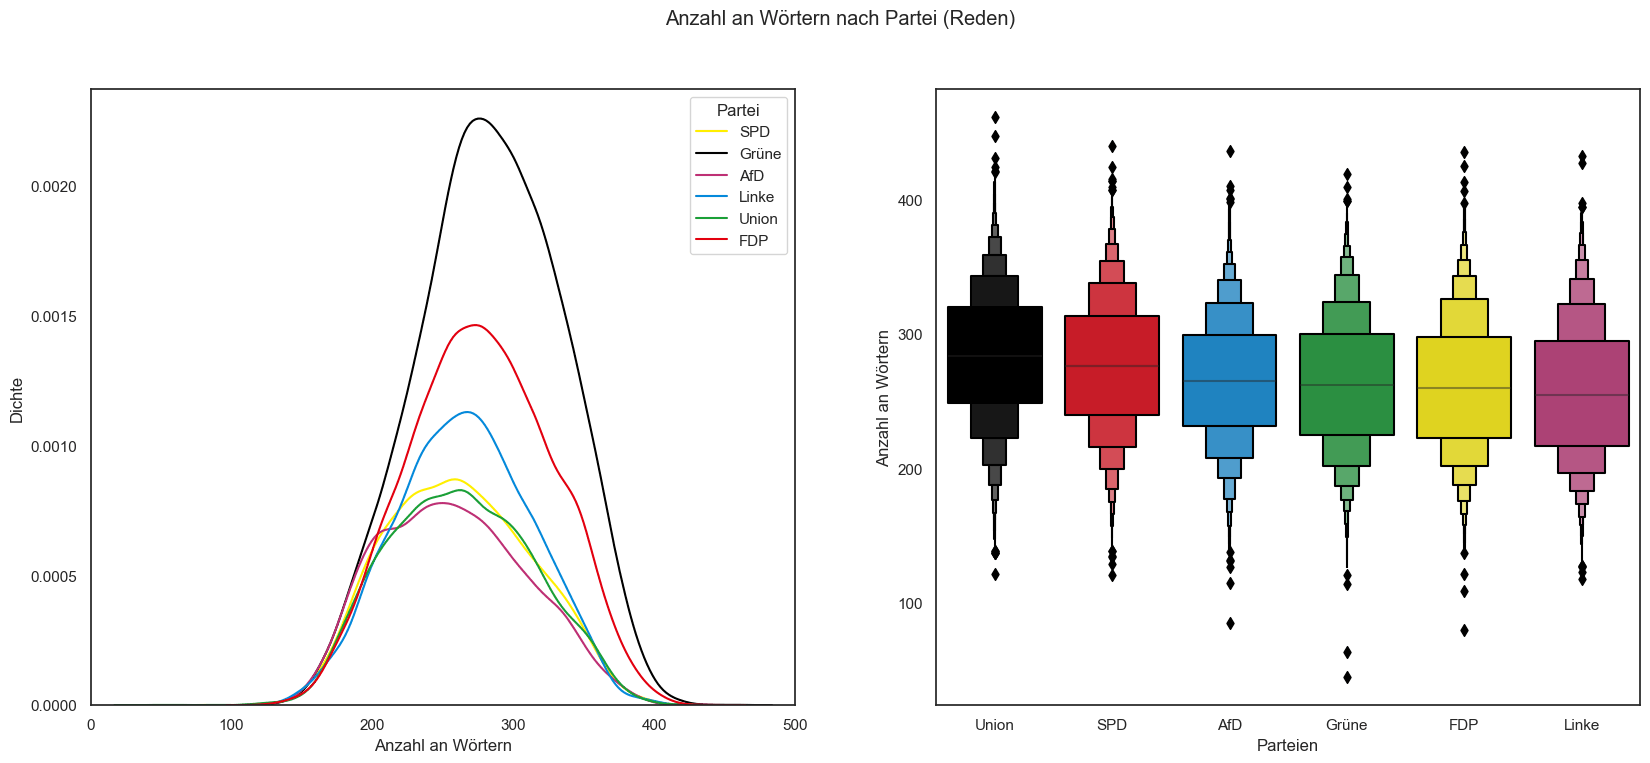
\includegraphics[width=0.9\textwidth]{data/images/speeches/speeches_word_count_after_filter.png}
    \caption{Anzahl an Wörtern für Reden nach Bereinigung} \label{fig:speechesWortCountAfterFiltering}
\end{figure}

\autoref{fig:speechesWortCountAfterFiltering} zeigt die Verteilung der Wortanzahl in den Reden pro Partei nach der Bereinigung und der Filterung. Es kann erkannt werden, dass es im Vergleich zu vor der Bereinigung (siehe \autoref{fig:wordCoundSpeeches}) keine Häufung von Reden unter \num{200} Wörtern mehr gibt.\footnote{Es ist möglich, dass es weiterhin Reden mit dieser Länge gibt, da die Untergrenze von \num{200} Wörtern vor weiteren -- eventuell kürzenden -- Bereinigungsschritten angewandt wird.} Je nach Partei schwankt der Hochpunkt der Verteilung zwischen \num{250} und \num{300} Wörtern. Es gibt kaum noch Redetexte über \num{400} Wörtern, da zu lange Reden aufgetrennt worden sind. Weiterhin sind die Reden der Union im Durchschnitt am längsten. Während die Redetexte der Grünen vor der Bereinigung am kürzesten sind, sind nun die der \ac{FDP} und der Linken kürzer, wenn auch nur marginal.

\begin{figure}[H]
    \centering
    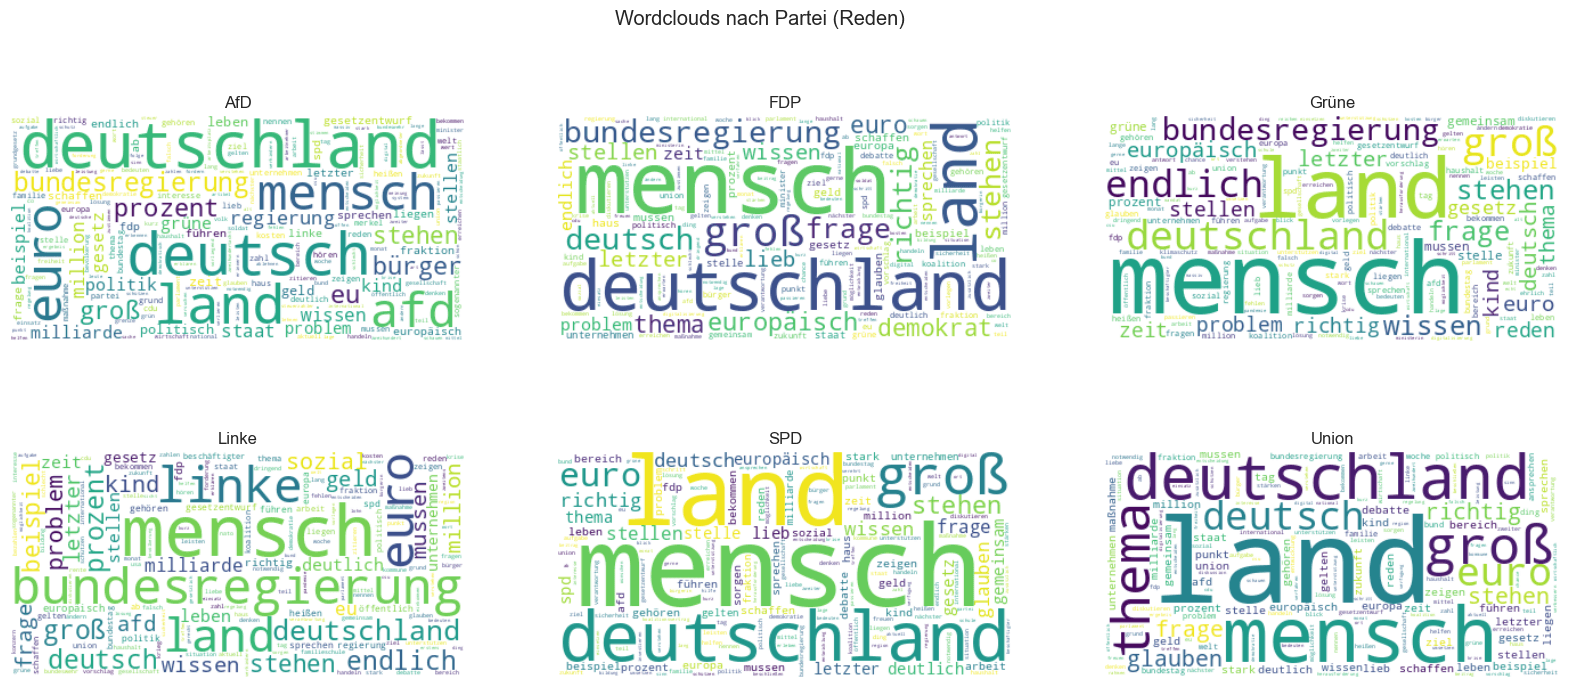
\includegraphics[width=0.9\textwidth]{data/images/speeches/speeches_wordclouds.png}
    \caption{Wortwolken mit den meistgenutzten Wörtern in Reden pro Partei} \label{fig:speechesWordclouds}
\end{figure}

Bei Betrachtung der meistgenutzten Wörter pro Partei, wie in \autoref{fig:speechesWordclouds} mittels Wortwolken dargestellt, fällt auf, dass jede Partei andere Schwerpunkte setzt und dabei ein anderes Vokabular nutzt. Die \ac{AfD} zeigt durch die häufige Nutzung der Wörter \textit{deutsch} und \textit{deutschland} ihren Fokus auf Nationalität, wobei auch bei der \ac{FDP}, \ac{SPD} sowie Union das Wort \textit{deutschland} zahlreich auftritt. Bei allen Parteien kommt das Wort \textit{euro} vor. \ac{FDP}, \ac{SPD} und Grüne nutzen zudem das Wort \textit{europäisch} häufig in ihren Reden. Besonders die Oppositionsparteien nutzen das Wort \textit{bundesregierung}, während die Regierungsparteien -- \ac{SPD} und Union -- dieses nur nachrangig verwenden. Daran lässt sich bestätigen, dass die Oppositionsparteien die Bundesregierung in ihren Reden oft direkt adressieren.

\begin{table}[H]
    \centering
    \caption{Prozentuale Sentimentverteilung von Reden pro Partei} \label{tab:sentimentDistributionSpeeches}
    {\footnotesize
    \begin{tblr}{width=\textwidth, hline{1-2, Z} = {0.75pt}, colspec={l*{3}{Q[si={table-format=1.2},c]}}, row{1}={guard,font=\bfseries,l}} 
        Partei & Negativ & Neutral & Positiv \\
        
        AfD & 0.45 & 0.54 & 0.01 \\
        Grüne & 0.48 & 0.50 & 0.02 \\
        Linke & 0.48 & 0.51 & 0.01 \\
        FDP & 0.41 & 0.57 & 0.02 \\
        \hline
        SPD & 0.22 & 0.75 & 0.03 \\
        Union & 0.19 & 0.78 & 0.02 \\
    \end{tblr}
    }
\end{table}

Um einen ersten Eindruck über die Ausrichtung der Reden zu bekommen, werden die Redetexte pro Partei mit einer Sentiment-Analyse untersucht. \autoref{tab:sentimentDistributionSpeeches} zeigt diesbezüglich die Verteilung der Reden mit negativem, neutralem und positivem Sentiment pro Partei. Es lässt sich ein starkes Gefälle zwischen den Regierungsparteien im Untersuchungszeitraum -- SPD und Union -- und den übrigen Oppositionsparteien erkennen: Während der Anteil mit negativem Sentiment bei den Regierungsparteien \SI{22}{\percent} und \SI{19}{\percent} beträgt, liegt dieser bei den Oppositionsparteien mit \SIrange{41}{48}{\percent} deutlich höher. Das könnte darauf zurückzuführen sein, dass Redner der Oppositionsparteien eher kritisch den Debatten gegenüberstehen, wohingegen Redner der Regierungsparteien hinter ihren Vorschlägen stehen und diese verteidigen.

\subsection*{Wahlprogramme}

Durch die Bereinigung und Filtern reduziert sich die Anzahl an Datenpunkten nur marginal. In dem Prozess werden einige Duplikate entfernt.

\begin{figure}[H]
    \centering
    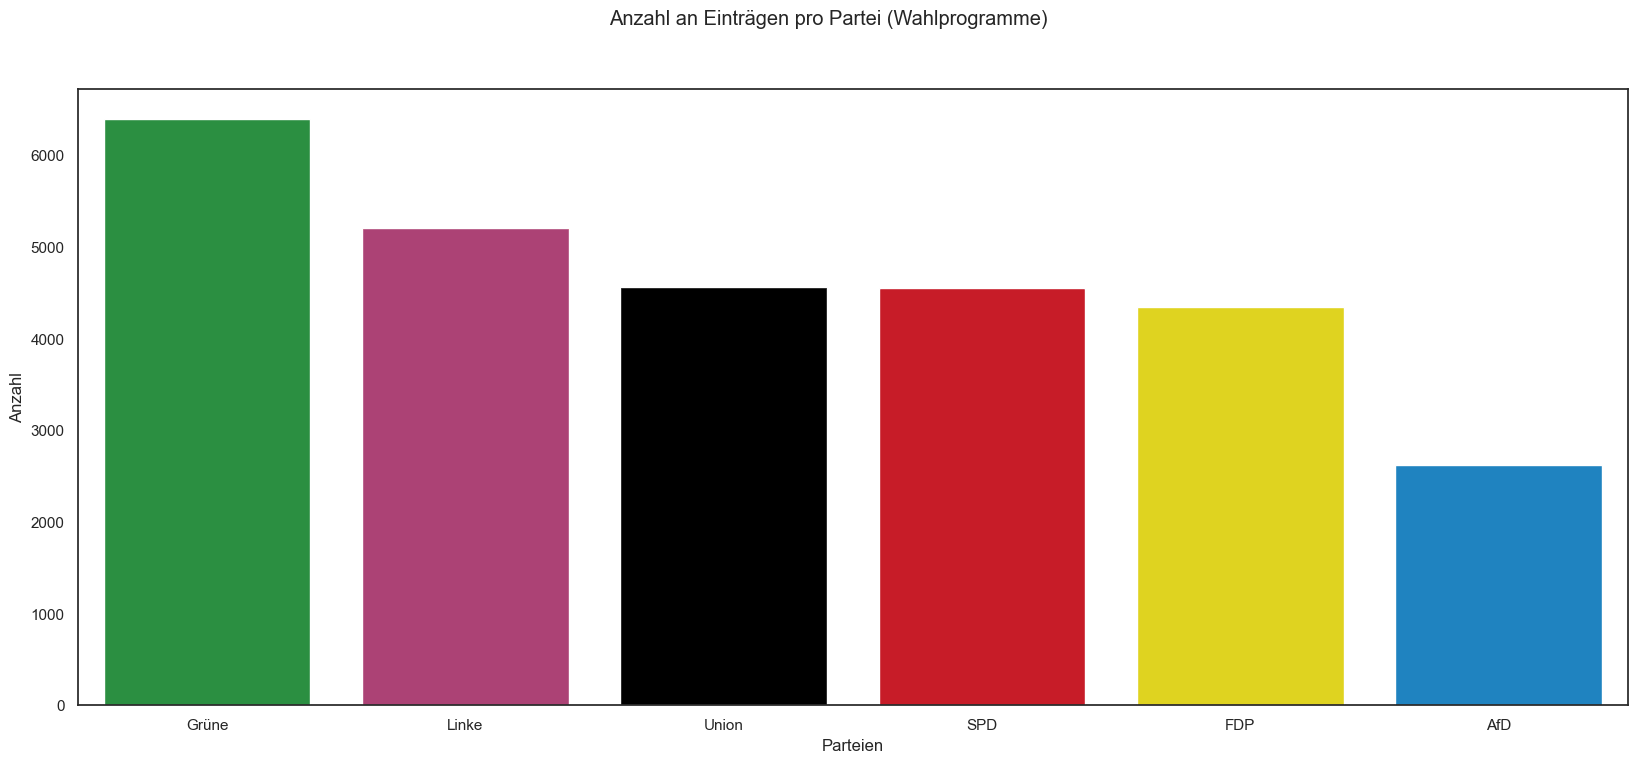
\includegraphics[width=0.9\textwidth]{data/images/party_programs/party_programs_num_samples_after_filter.png}
    \caption{Anzahl an Einträgen für Wahlprogramme pro Partei nach Bereinigung} \label{fig:partyProgramsNumSamplesAfterFiltering}
\end{figure}

Die Anzahl an Einträgen im Wahlprogramm-Datensatz pro Partei, wie in \autoref{fig:partyProgramsNumSamplesAfterFiltering} dargestellt, zeigt, dass von den Grünen mit über \num{6000} am meisten vorliegen, gefolgt von gut \num{5000} von der Linken. Union, \ac{SPD} und \ac{FDP} liegen mit ca. \num{4500} gleich auf. Mit Abstand am wenigsten Absätze -- nämlich \num{2600} -- liegen von der \ac{AfD} vor, da es dort bei sechs Wahlen zu Problemen mit dem Auslesen des Wahlprogramm-Textes aus der \ac{PDF}-Datei gekommen ist.

\begin{figure}[H]
    \centering
    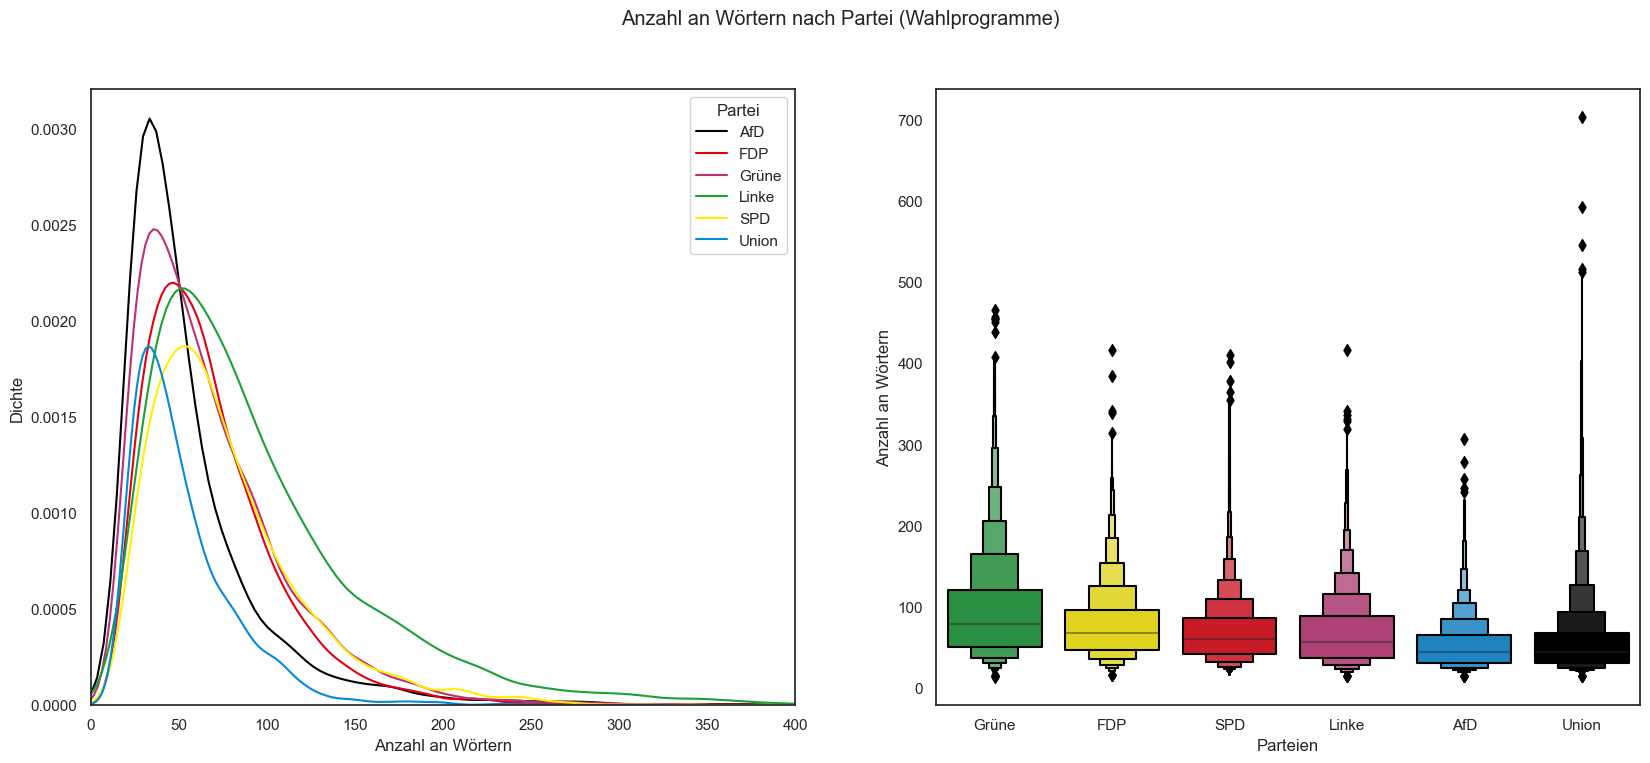
\includegraphics[width=0.9\textwidth]{data/images/party_programs/party_programs_word_count_after_filter.png}
    \caption{Anzahl an Wörtern für Wahlprogramme nach Bereinigung} \label{fig:partyProgramsWordCountsAfterFiltering}
\end{figure}

\autoref{fig:partyProgramsWordCountsAfterFiltering} zeigt die Verteilung der Wortanzahl in den Wahlprogramm-Absätzen pro Partei nach Bereinigung und Filterung. Es ergeben sich keine grundlegenden Unterschiede im Vergleich zur Verteilung vor der Bereinigung. Weiterhin ist eine Häufung von Reden, die etwa \num{50} Wörter umfassen, festzustellen. Dabei liegen die verschiedenen Parteien etwa gleich auf, mit den längsten Paragraphen bei den Grünen und den kürzesten bei der Union.

\begin{figure}[H]
    \centering
    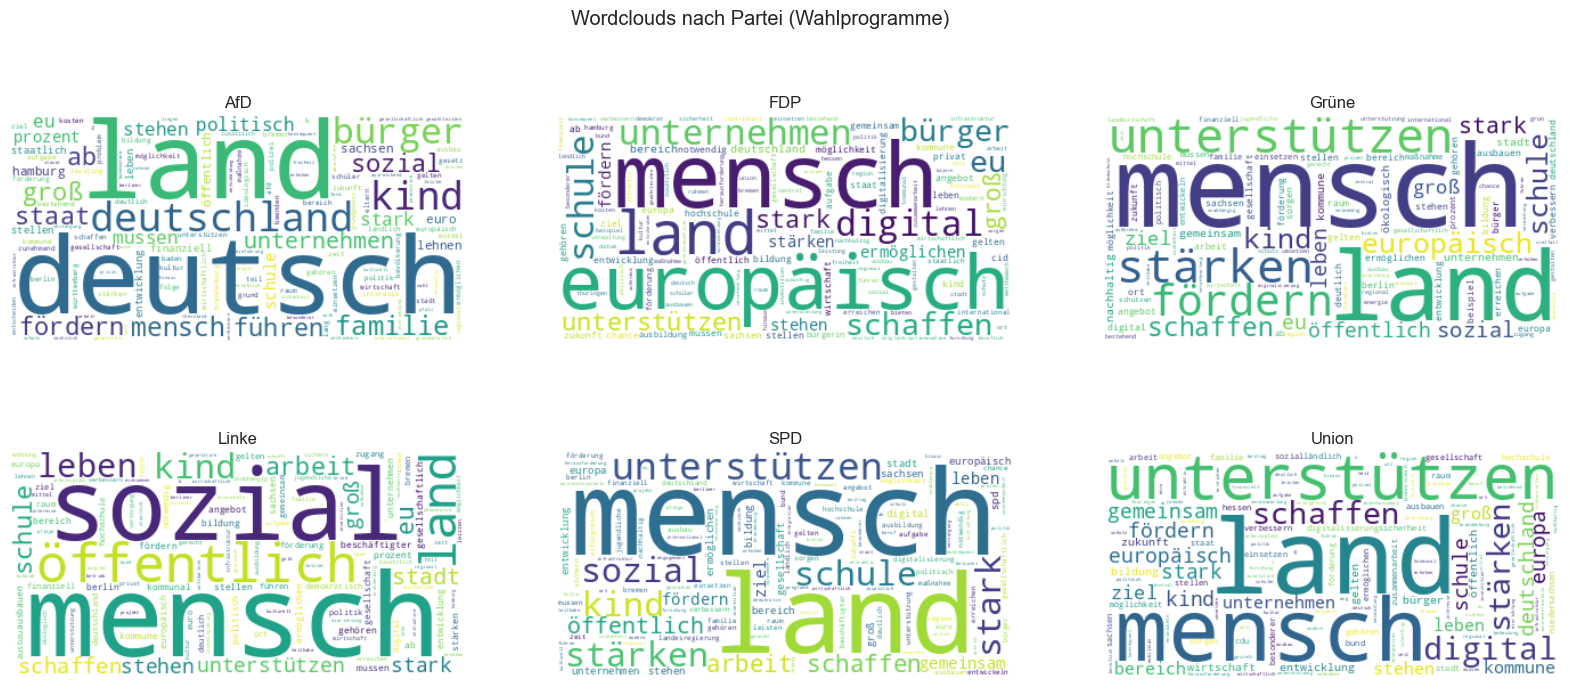
\includegraphics[width=0.9\textwidth]{data/images/party_programs/party_programs_wordclouds.png}
    \caption{Wortwolken mit den meistgenutzten Wörtern in Wahlprogrammen pro Partei} \label{fig:partyProgramsWordclouds}
\end{figure}

Auch bei den Wahlprogrammen lassen sich einige Erkenntnisse anhand der Wortwolken mit den meistgenutzten Wörtern ableiten, die in \autoref{fig:partyProgramsWordclouds} dargestellt sind. Ähnlich wie in den Reden, verwendet die \ac{AfD} je nach Kontext als patriotisch geltende Wörter wie \textit{land}, \textit{deutsch} oder \textit{deutschland}. Anhand viel genutzter Wörter der \ac{FDP} wie \textit{europäisch}, \textit{unternehmen} oder \textit{digital} spiegeln sich Schwerpunkte der Partei wie Wirtschaftsliberalismus und Digitalpolitik sowie eine proeuropäische Haltung wider. Begriffe wie \textit{sozial} und \textit{öffentlich} deuten auf den sozialpolitischen Fokus der Linken hin. Die \ac{SPD} legt einen Fokus auf unter anderem Sozial- und Bildungspolitik (\textit{sozial} sowie \textit{schule}). Grüne und Union nutzen ähnliche Begriffe wie \textit{mensch}, \textit{land} und \textit{unterstützen} am häufigsten. Die Begriffe können je nach Partei unterschiedlich ausgelegt werden.

\begin{table}[H]
    \centering
    \caption{Prozentuale Sentimentverteilung von Wahlprogrammen pro Partei} \label{tab:sentimentDistributionPartyPrograms}
    {\footnotesize
    \begin{tblr}{width=\textwidth, hline{1-2, Z} = {0.75pt}, colspec={l*{3}{Q[si={table-format=1.2},c]}}, row{1}={guard,font=\bfseries,l}} 
        Partei & Negativ & Neutral & Positiv \\
        
        AfD & 0.03 & 0.97 & 0.00 \\
        Grüne & 0.03 & 0.96 & 0.01 \\
        Linke & 0.05 & 0.95 & 0.00 \\
        FDP & 0.02 & 0.97 & 0.01 \\
        \hline
        SPD & 0.01 & 0.98 & 0.01 \\
        Union & 0.01 & 0.98 & 0.01 \\
    \end{tblr}
    }
\end{table}

Die Auswertung des Sentiments in den Wahlprogramm-Texten des Datensatzes, die in \autoref{tab:sentimentDistributionPartyPrograms} gezeigt ist, ergibt, dass die Wahlprogramme primär in neutraler Stimmung formuliert sind (bei jeder Partei mindestens \SI{95}{\percent}). Die größte Abweichung davon zeigt die Linke, deren Wahlprogramme zu einem Anteil von \SI{5}{\percent} als negativ kategorisiert werden. Wahlprogramme werden als informative Schriftstücke verfasst werden, während bei Reden und Tweets mit anderen Personen diskutiert wird und so oft ein eindeutiges Sentiment vorherrscht. Daher erklärt sich der geringe Anteil an Textabschnitten in Wahlprogrammen, denen eine negative oder positive Gesinnung attestiert wird.

\section{Fazit} \label{sec:crispConclusion_1}

Für das Training der Klassifikationsmodelle werden Datensätze aus drei Textsorten genutzt: Tweets, Wahlprogramme und Reden. Der Tweet-Datensatz enthält mehr Einträge als die anderen beiden, wobei die Dokumentlänge der einzelnen Einträge deutlich kürzer ist. Für jeden Datensatz werden verschiedene Schritte zur Datenbereinigung durchgeführt. Zuerst erfolgen regelbasierte Verfahren, dann werden alle Wörter auf ihren Wortstamm reduziert und schließlich werden Stopwörter entfernt. Zu den regelbasierten Verfahren gehört auch das Umwandeln von gegenderten Formen zum generischen Maskulinum, da anderenfalls die Wortstammbildung nicht korrekt durchgeführt werden kann. Im Anschluss an die Datenbereinigung werden Duplikate und zu kurze Texte gefiltert. Im Reden-Datensatz müssen zu lange Texte in mehrere Einträge aufgespalten werden.

Nach den dargelegten Aufbereitungsschritten bleiben vorwiegend im Tweet-Datensatz bedeutend weniger Einträge übrig. Die Anzahl der Wahlprogramm-Paragraphen bleibt gleich und es liegen mehr Reden -- genauer gesagt Teile von Reden -- vor. Eine erste Analyse mittels Wortwolken zeigt, dass Politiker in ihren Tweets in hoher Zahl ihre eigene Partei nennen. In den Reden und Wahlprogrammen liegt der Fokus auf den thematischen Schwerpunkten der jeweiligen Partei. Die Analyse des Sentiments der Texte legt offen, dass Tweets und Reden überwiegend neutral oder negativ gestimmt sind. Auffällig ist, dass die Regierungsparteien (\ac{SPD} und Union) deutlich weniger negative Einträge veröffentlichen als die Opposition. Wahlprogramme sind der Analyse nach fast ausschließlich neutral verfasst.